% Assessment of transfer methods

\chapter{Assessment of transfer methods for comparative genomics of regulatory
  networks in Bacteria}

\section{Background}

The availability of complete genome sequences for related organisms can be
effectively leveraged to study transcriptional regulatory networks (TRN)
\cite{babu2008computational}. In the past decade, comparative genomics
approaches have been routinely employed to study bacterial transcriptional
regulatory networks, or regulons, controlled by a single transcription factor
(TF). These studies have enabled the identification of core network elements
and niche-specific adaptations, providing insights into the evolution of these
systems~\cite{tan2001comparative, makarova2001conservation,
  erill2004differences, venancio2009reconstructing, baumbach2010power,
  rodionov2013transcriptional}. A conventional TRN comparative genomics
analysis typically involves three well-defined steps
\cite{babu2008computational, gelfand2000comparative, baumbach2009reliable}. The
first step consists in the transfer of available information on the regulatory
network (i.e.\ known TF-binding sites and/or regulated genes) to the species
under analysis, in order to infer the TF-binding motif in these target
species. The second step involves a genome-wide search for putative TF-binding
sites in the target genomes using the inferred TF-binding motifs. In the third
step, search results from multiple genomes are integrated across orthologs,
based on the assumption that only orthologs of regulated genes will
systematically display TF-binding sites in their promoter regions.

The power of comparative genomics arises from the aggregation of predictions in
multiple genomes under the assumption of functional selection, which
dramatically reduces the number of false positives
\cite{gelfand2000comparative}. However, the effectiveness of this approach
depends crucially on the success of the initial transfer step. Information from
a reference TRN can be transferred through the assumption of a conserved
TF-binding motif, a conserved regulon, or a combination of the two
\cite{babu2008computational, baumbach2010power}. As a consequence, several
methods have been proposed to transfer regulatory information across
species. The simplest approach, here called “direct transfer”, is to use the
reference TF-binding motif to search for sites in the target genome. The target
motif is hence implicitly defined as a subset of the highest scoring sites in
that genome~\cite{tan2001comparative, makarova2001conservation,
  erill2004differences, rodionov2013transcriptional}.
The direct transfer scheme can be further elaborated by applying a motif discovery
or optimization algorithm (``direct discovery'')
on a set of high-scoring sites from the target genome
\cite{baumbach2009reliable, habib2012functional}. The alternative to TF-binding
motif-based transfer is to assume conservation of gene content in the
TRN\@. Such regulon or “network transfer” is typically implemented through the
detection of orthologs for genes in known regulated operons. The promoter
regions of the corresponding operons in target genomes are then analyzed with a
motif discovery tool to elicit the TF-binding motif
\cite{mccue2001phylogenetic, wang2003combining, panina2003comparative,
  zhang2009genome}. If network information is not available, a minimal network
consisting only of the TF-coding gene can be postulated under the assumption of
self-regulation, and the TF-binding motif can be inferred with motif discovery
tools applied to the promoter region of the TF-coding gene
\cite{francke2008generic, cornish2012inference,
  ravcheev2014comparative}. Lastly, motif- and network-based transfer
approaches can be combined in “mixed transfer” to minimize false positives, at
the expense of lowered sensitivity~\cite{baumbach2010power,
  baumbach2009reliable, yu2004annotation}.

The limited availability of experimental data on TF-binding sites has hindered
attempts at systematically assessing and comparing methods for transfer of
transcriptional regulatory networks. Early studies on TRN transfer indicated
that the efficiency of methods based on TF-binding motif transfer faced a sharp
drop-off with increasing sequence divergence among the TF orthologs
\cite{yu2004annotation}. Later studies exposed the limitations of network-based
transfer methods, due to shortcomings in orthology detection methods and the
flexible nature of bacterial TRNs~\cite{babu2006evolutionary,
  chavez2006bacterial, price2007orthologous}. It has been suggested that mixed
transfer methods provide better results~\cite{baumbach2010power}, but the
scarcity and distributed nature of TF-binding site data have to date prevented
systematic benchmarking of these methods. Here we report the mining
and integration of experimental TF-binding site data from multiple databases
into a unified catalog. Leveraging this resource, we performed a systematic
evaluation of TRN transfer methods across pairs of species and using multiple
metrics. In agreement with previous reports, our results reveal that
motif-based transfer methods perform best, but decay sharply at high TF
sequence divergence. In contrast, the efficiency of network-based transfer
methods is poor and weakly dependent of phylogenetic distance, while mixed
methods do not significantly improve the results of motif-based transfer
methods. Our analysis also highlights the inadequacy of
receiver-operating-characteristic (ROC) curves in heavily unbalanced settings
and indicates that the precision-recall (PR) area-under-the-curve (AUC) is the
most informative statistic for assessment of transfer results. We evaluate
predictive measures for transfer accuracy and discuss their applicability in
the context of comparative genomics analysis.


\section{Results and Discussion}

\subsection{Data compilation and evaluation of metrics for the assessment of
  transfer methods}

To perform a systematic analysis of methods for the transfer of transcriptional
regulatory networks in Bacteria, we compiled data from five major databases
reporting experimentally-validated TF-binding sites across the Bacteria
domain. After consolidating replicates, we obtained a catalog of 7,603
TF-binding sites for 344 TFs in 166 species
(Table~\ref{tab:database-numbers}). To analyze TRN transfer, we focused on
TF/species pairs that contained at least 10 binding sites for the same TF in
both species. The resulting dataset contains 179 TF-specific species pairs for
15 different TFs across 35 bacterial species and is dominated by instances of
the global transcriptional regulators LexA and Fur
(Table~\ref{tab:number-of-species-pairs}).

\begin{table}
\caption{Distribution of TF-binding sites in the compiled catalog by
originating database.}
\label{tab:database-numbers}
\centering
\begin{tabular}{l r}
\toprule
Database & Number of binding sites \\
\midrule
CollecTF~\cite{kilic2013collectf} & 4,942 \\
DBTBS~\cite{sierro2008dbtbs} & 116 \\
MtbRegList~\cite{jacques2005mtbreglist} & 202 \\
CoryneRegNet~\cite{pauling2012coryneregnet} & 196 \\
RegulonDB~\cite{salgado2013regulondb} & 2,147 \\
\bottomrule
\end{tabular}
\end{table}

\begin{table}
\centering
\caption{Distribution by TF of the number of species pairs with at least 10
  experimentally validated TF-binding sites in each species.}
\label{tab:number-of-species-pairs}

\begin{tabular}{l r}
\toprule
TF & Number of species pairs \\
\midrule
  Fur & 154 \\
  LexA & 134 \\
  CcpA & 20 \\
  PhoP & 12 \\
  CodY & 12 \\
  OmpR & 6 \\
  CRP & 4 \\
  RpoN & 4 \\
  FNR & 2 \\
  PurR & 2 \\
  DtxR & 2 \\
  ArgR & 2 \\
  PvdS & 2 \\
  CsgD & 2 \\
\bottomrule
\end{tabular}
\end{table}

The establishment of an adequate metric is a necessary and crucial element in a
benchmark study. When transferring TRNs from a reference species to a target
species for comparative genomics, the result of the transfer process is an
inferred TF-binding motif in the target species. Given the inferred and known
TF-binding motifs in the target genome, one can evaluate the accuracy of the
transfer process by directly comparing the motifs or by assessing the
efficiency of the inferred motif at retrieving the known TF-binding sites in a
genome search. Here we focused on the Euclidean distance and the
Kullback–Leibler (KL) divergence as well-established motif comparison functions
based on the position-specific frequency matrix (PSFM) defined by the motif
\cite{gupta2007quantifying}, and on two standard metrics for classification
accuracy based on the area-under-the-curve (AUC) derived from a TF-binding site
search process: the receiver-operating-characteristic (ROC) AUC and the
precision-recall (PR) AUC~\cite{lewis1991evaluating, zweig1993receiver}. To
assess the efficacy of each method at discriminating the effectiveness of TRN
transfer, we simulated transfers by defining inferred motifs as noisy
pseudo-replicates or permutations of the known collection of binding sites in
the target genomes (Figure~\ref{fig:pseudoreplicate-generation}). We then
assessed the quality of these simulated transfers against the known target
motif using the four metrics outlined above
(Figure~\ref{fig:transfer-evaluation-comparison}).

\begin{figure}
  \centering
  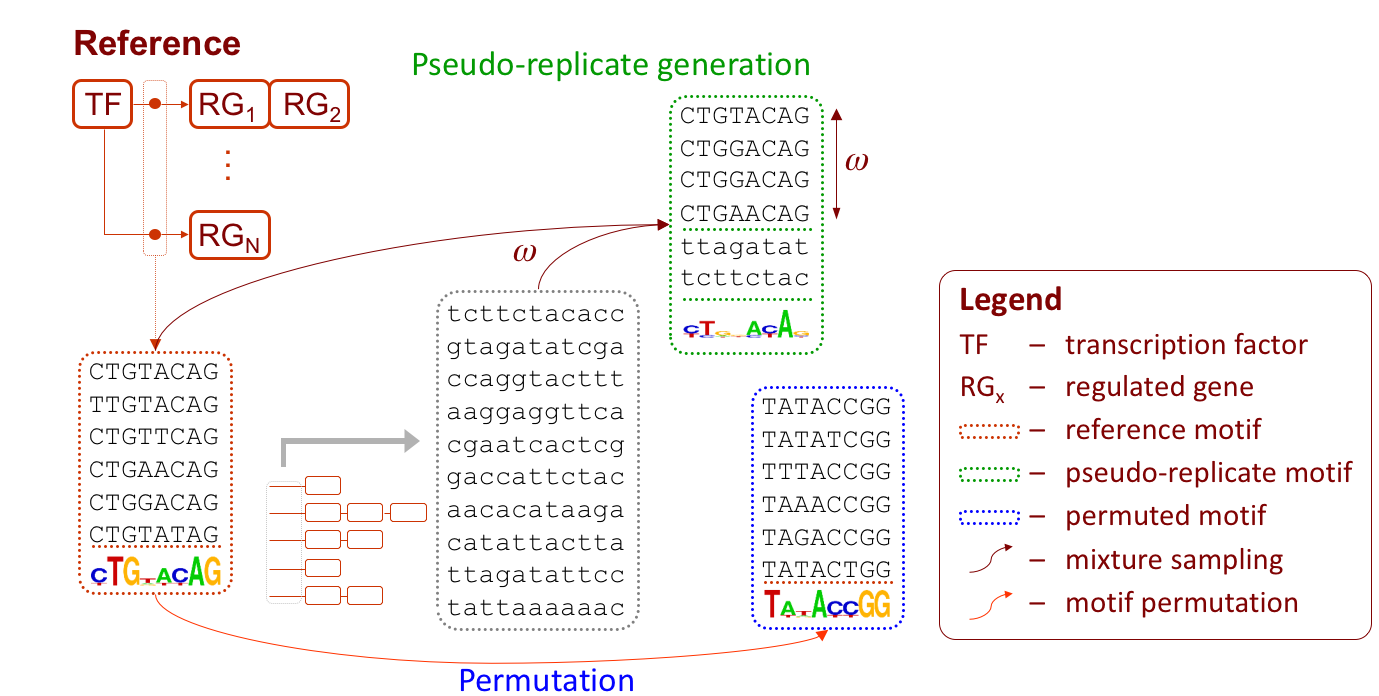
\includegraphics[width=\textwidth]{figures/chapter3/pseudoreplicate-generation}
  \caption{Generation of noisy transfers and controls as mixture
    pseudo-replicates or permuted motifs. Pseudo-replicates of the same size as
    the original reference collection are generated by randomly sampling, with
    replacement, the reference collection and promoter sequences of equivalent
    length from the reference genome using a mixture weight $\omega$. Permuted
    motifs are generated by sampling, without replacement, the columns of the
    reference collection.}
\label{fig:pseudoreplicate-generation}
\end{figure}

As it can be seen in Figure~\ref{fig:transfer-evaluation-comparison}, both the
Euclidean distance and KL-divergence perform only moderately well at
discriminating the results of simulated noisy transfers (containing 50\% and
75\% random sites) from completely random or permuted motifs. This result is
partly due to the fact that the expectation for random motifs is not to yield maximum
distance, narrowing the useful range of motif comparison metrics. The two other
contributing factors are the high-dimensionality of TF-binding motifs, which is
known to decrease the relative contrast of
L-norms~\cite{aggarwal2001surprising}, and the presence of low information
bearing positions in most TF-binding motifs. Low information positions are
intrinsically close in PSFM space, artificially increasing the similarity
between motifs for both metrics~\cite{zhang2013spic}. As a result, in both
cases, random and permuted motifs display a considerable spread, leading to
significant overlap with the results obtained for simulated noisy transfers. In
practice, transfer methods frequently generate motifs comparable to the noisy
transfers simulated here, and their overlap with random controls therefore
complicates the interpretation of transfer results.

\begin{figure}
  \centering
  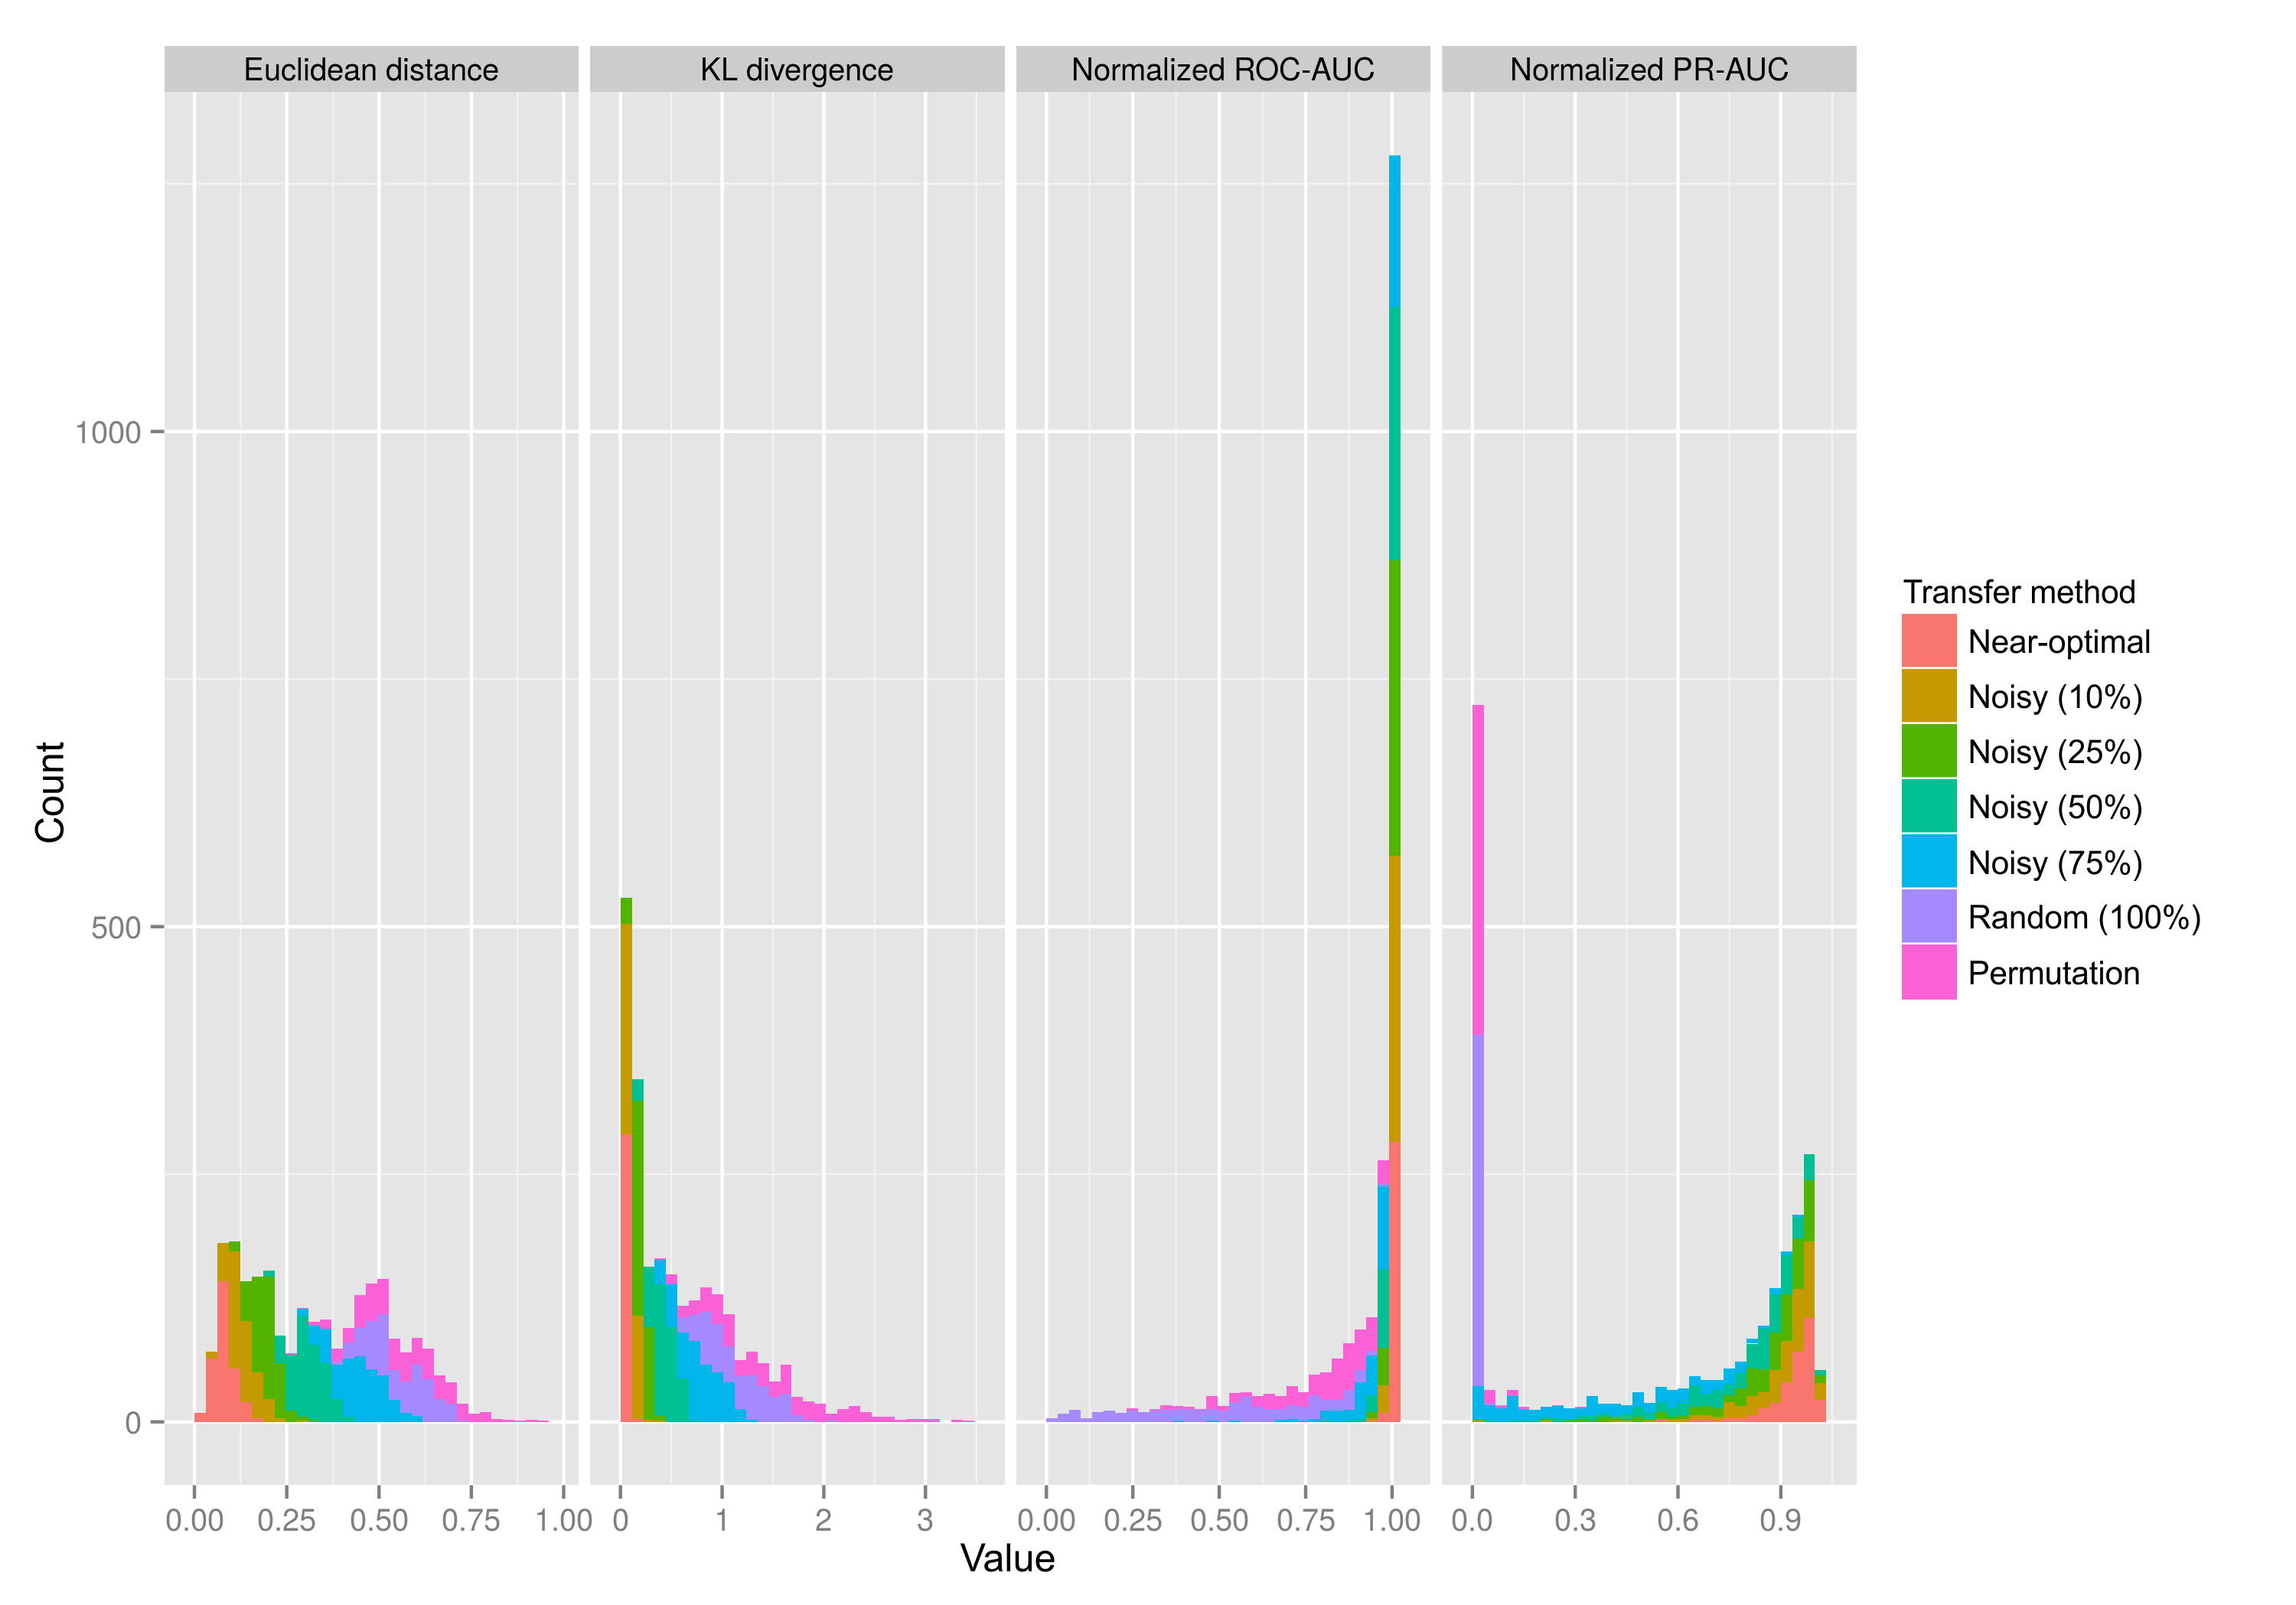
\includegraphics[width=0.9\textwidth]{figures/chapter3/transfer-evaluation-comparison}
  \caption{Comparison of methods for the evaluation of TRN transfer. The plots
    show the histogram of Euclidean distance, KL divergence, ROC-AUC and PR-AUC
    values for simulated bidirectional transfers between 179 TF-specific
    species pairs using different degrees of noise (10, 25, 50 and 75\% of
    random sites sampled when creating pseudo-replicates), as well as their
    random and permuted controls. The y-axis shows the number of transfers
    within each binning value on the x-axis. ROC-AUC and PR-AUC values are
    normalized to the respective AUC of the known target TF-binding motif to
    compensate for the decreased search efficiency of low information content
    motifs.}
\label{fig:transfer-evaluation-comparison}
\end{figure}

Accuracy metrics based on a genome-wide search for known TF-binding sites
should in principle provide a more informative metric of the effectiveness of
the transfer process since they evaluate the ability of the inferred motif to
locate true binding sites in the target genome. In contrast with motif
comparison methods, the expectation for accuracy metrics is hence that
incorrect or random transfers should yield very low AUC values. However, this
does not happen for the ROC-AUC, a widely adopted metric in bioinformatics
\cite{saito2015precision}. This result is due to the large class imbalance in
the TF-binding search problem, where a handful of known true sites must be
distinguished from the genome background. Even though ROC curves scale properly
with class imbalance~\cite{fawcett2006introduction}, they are ill-suited to
discriminate between classifiers in a heavily imbalanced context, because the
negative class dominates the computation of the ROC-AUC
\cite{davis2006relationship}. The net result of this effect is a compression of
AUC scores for noisy motifs into a very narrow range (0.9--1.0), making
discrimination between near-optimal and noisy transfers almost impossible. This
compression also affects the results obtained for random and permuted motifs,
which spread all the way up to 0.95 AUC scores, further complicating the
interpretation of transfer results. By focusing on the ratio of true and false
positives (precision) and otherwise ignoring the negative class, the PR-AUC
generates scores are not compressed by class imbalance
\cite{saito2015precision, davis2006relationship}. As it can be seen in
Figure~\ref{fig:transfer-evaluation-comparison}, the PR-AUC effectively
exploits its range to discriminate between noisy transfers and systematically
assigns very small values to random and permuted motifs. Hence, the PR-AUC
provides the most effective metric for the benchmarking of TRN transfer methods
and was used in all subsequent analyses reported here.

\subsection{Comparison of transfer methods}

Motif-based and network-based transfer methods rely on different assumptions
about the evolutionary dynamics of transcriptional regulatory networks. The
former assume that the TF-binding motif is conserved to some extent while the
latter assume that the gene components of the regulon are conserved. As a
result, it is presumed that motif-based methods will perform poorly at large
phylogenetic distances due to expected divergence in the TF-binding motif,
whereas network-based methods are expected to be more resilient to phylogenetic
distance if the biological function of the regulatory network is
preserved. Interestingly, there is evidence supporting and invalidating both
assumptions and their corollaries. The SOS response transcriptional regulator
LexA, for instance, has been shown to target widely diverging motifs in
relatively close species~\cite{erill2007aeons}, whereas some transcriptional
regulators, like the heat-shock response repressor HrcA or the arginine
repressor ArgR, are known to preserve their binding motif across Bacteria to
different extents~\cite{makarova2001conservation, gelfand1999recognition}. On
the other hand, regulon composition has been documented to vary significantly
even among closely related species~\cite{erill2004differences,
  venancio2009reconstructing, baumbach2010power,
  price2007orthologous}. Furthermore, CRP/FNR-type regulators have been shown
to control completely different networks using closely related motifs across
Bacteria~\cite{dufour2010reconstruction, matsui2013comprehensive}.

Here we tested the robustness of TRN transfer methods by evaluating the PR-AUC
of inferred TF-binding motifs in 179 TF-specific species pairs, using three
motif-based and three network-based methods, as well as a combination of motif-
and network-based methods (Figure~\ref{fig:transfer-methods}). The motif-based
transfer methods include direct transfer and direct discovery methods. In the
direct transfer, the reference collection of TF-binding sites is used directly
to determine the inferred collection by searching promoter regions in the
target genome. In direct discovery, the results of a relaxed search and their
surrounding regions are used as input for a motif discovery algorithm, with the
goal of generating a motif better adapted to the target genome. The
network-based transfer methods evaluated differ in how they map genes regulated
in the reference genome to the target genome. This mapping can be based on the
detection of direct orthology for genes in regulated operons, their functional
assignment using Clusters of Orthologous Groups (COGs) or orthology detection
using their interacting network partners. The mixed approach combines a relaxed
TF-binding motif search with the restriction that identified sites must be
associated with genes mapped with any of the three network-based transfer
approaches.

\begin{figure}
  \centering
  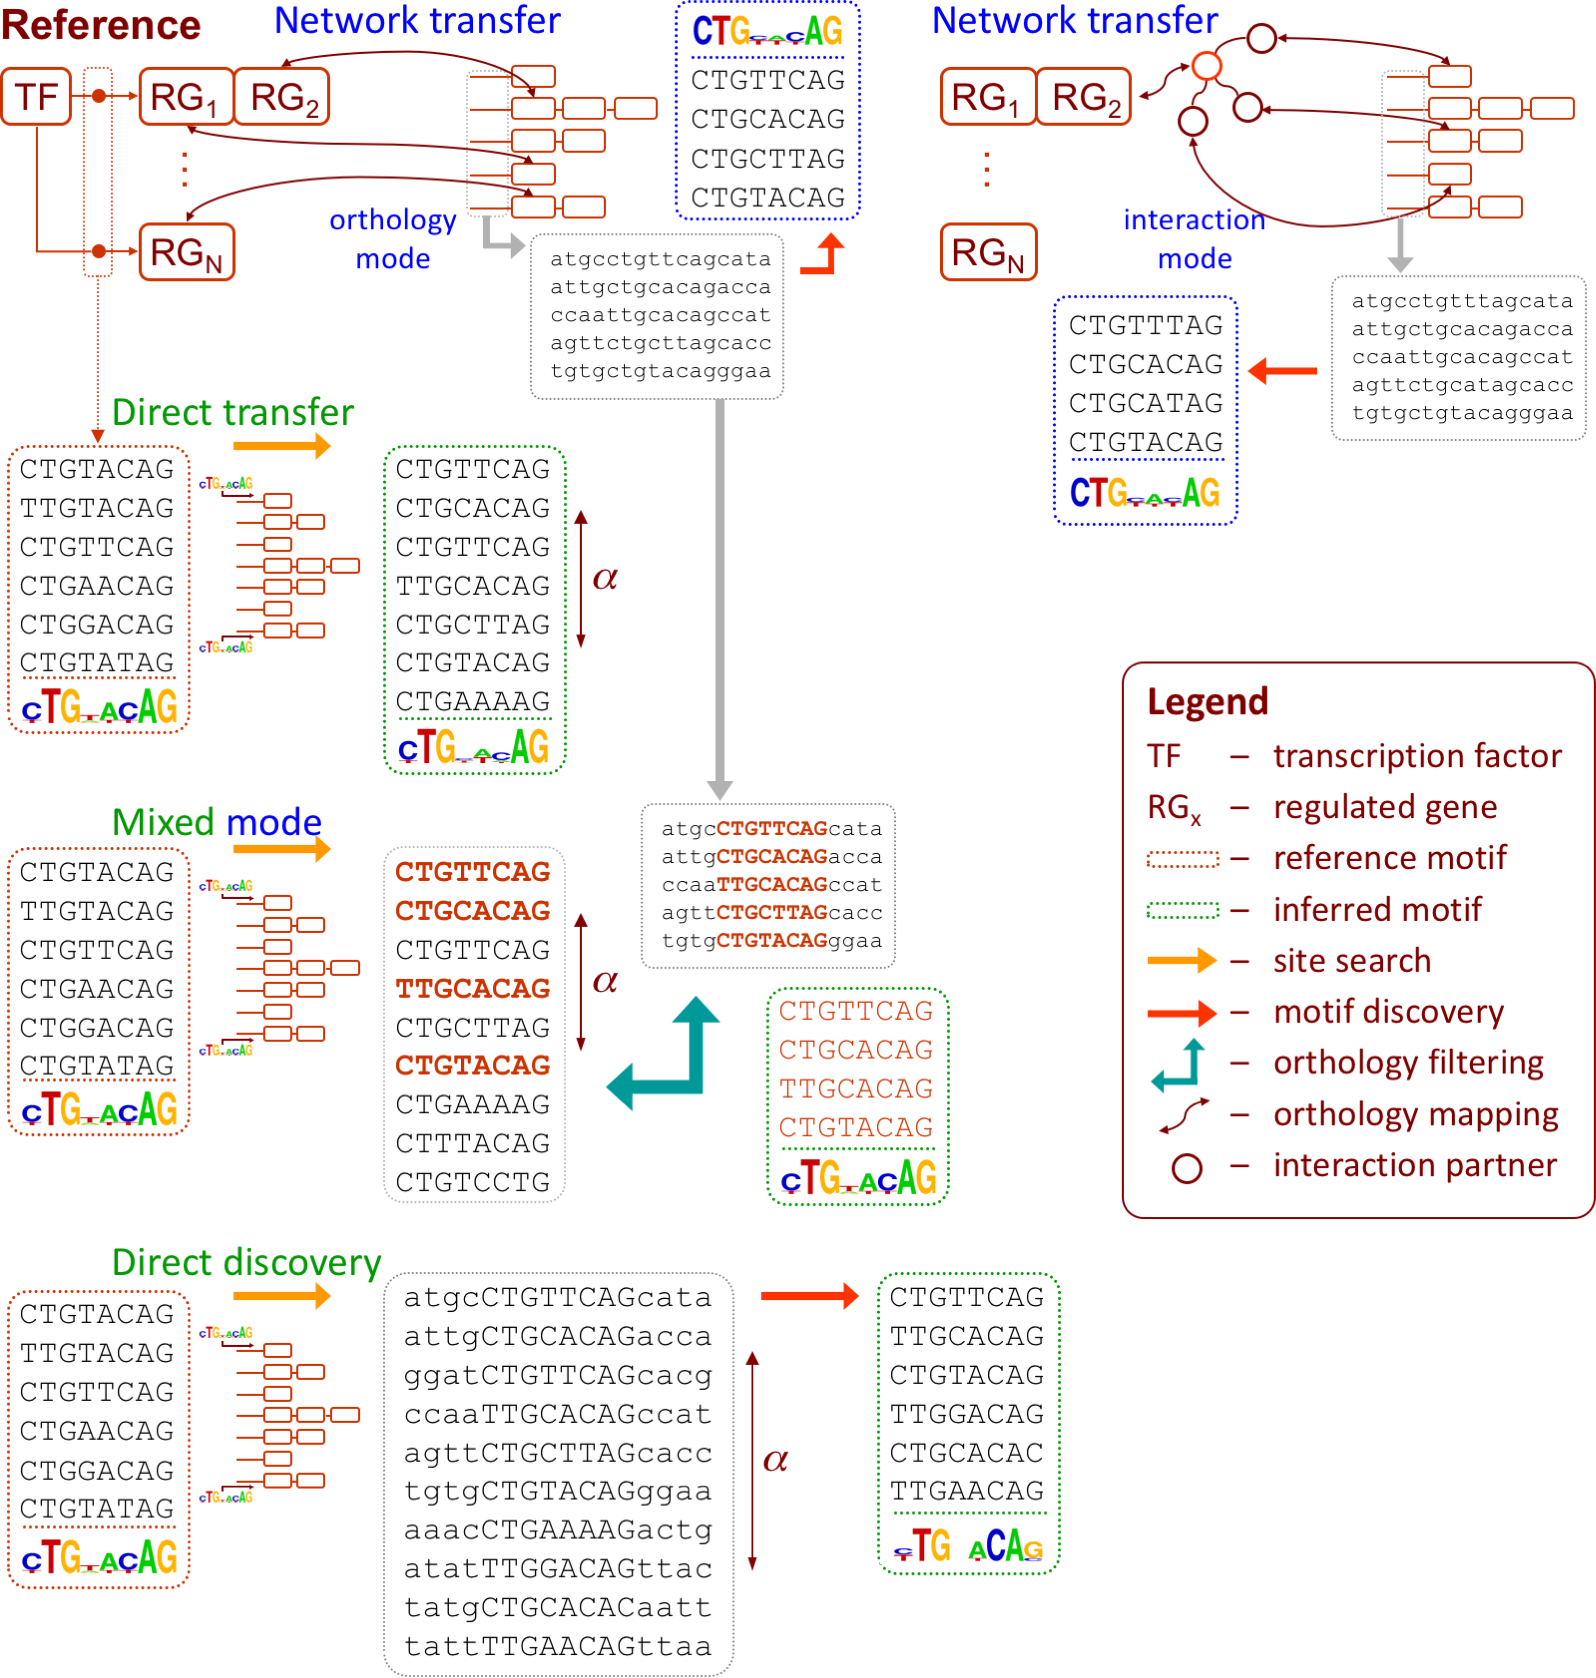
\includegraphics[width=\textwidth]{figures/chapter3/transfer-methods}
  \caption{Schematic representation of implemented transfer methods. The
    network-based COG mode and the motif-based direct discovery with true
    promoters are omitted.}
\label{fig:transfer-methods}
\end{figure}

In agreement with previous research, the results shown in
Figure~\ref{fig:comparison-transfer-methods} reveal that the effectiveness of
motif-based transfer methods declines rapidly with decreasing sequence
similarity between the TF protein sequences~\cite{yu2004annotation}. In
contrast, the results of network-based transfer methods show only moderate
correlation with protein sequence similarity, but these methods perform poorly
when compared to motif-based transfer methods. Among the three mapping modes
analyzed for network-based transfer, the direct ortholog mode provides the best
results but is still only able to generate successful transfers in 15\% of the
cases. The poor efficiency of network-based transfer methods supports previous
research highlighting the evolutionary flexibility of bacterial transcriptional
regulatory networks, which decreases their expected overlap in gene composition
\cite{venancio2009reconstructing, babu2006evolutionary, chavez2006bacterial,
  price2007orthologous}. The low efficiency of network-based transfers could,
therefore, stem from an inability of these transfer methods to identify
conserved regulated genes (low recall) or from the inclusion of too many
orthologs without conserved regulation in the transfer process (low
precision). The interplay between these factors should explain the significant
differences observed between network transfer modes since these variants are
intended to progressively relax the concept of orthology in order to enhance
recall. To analyze their relative contributions, we computed the Spearman
correlation coefficient between the search PR-AUC reported in
Figure~\ref{fig:comparison-transfer-methods} and the precision/recall of the
network transfer process for the different transfer modes. We find that recall
($\rho_r=0.115$), rather than precision ($\rho_p=0.106$), is the dominant
factor for the more restrictive ortholog mode. This indicates that detecting
enough orthologs with conserved regulation is critical for proper motif
inference. However, the situation is reversed for the more relaxed COG
($\rho_r=0.089$; $\rho_p =0.191$) and interaction ($\rho_r=-0.108$;
$\rho_p=0.140$) modes. These results suggest that the increase in mapped
orthologs that are not regulated in the target genome (loss of precision)
overcomes any substantial enhancement in recall achieved by relaxed mapping
modes (Figure~\ref{fig:network-transfer-auc}).

\begin{figure}
  \centering
  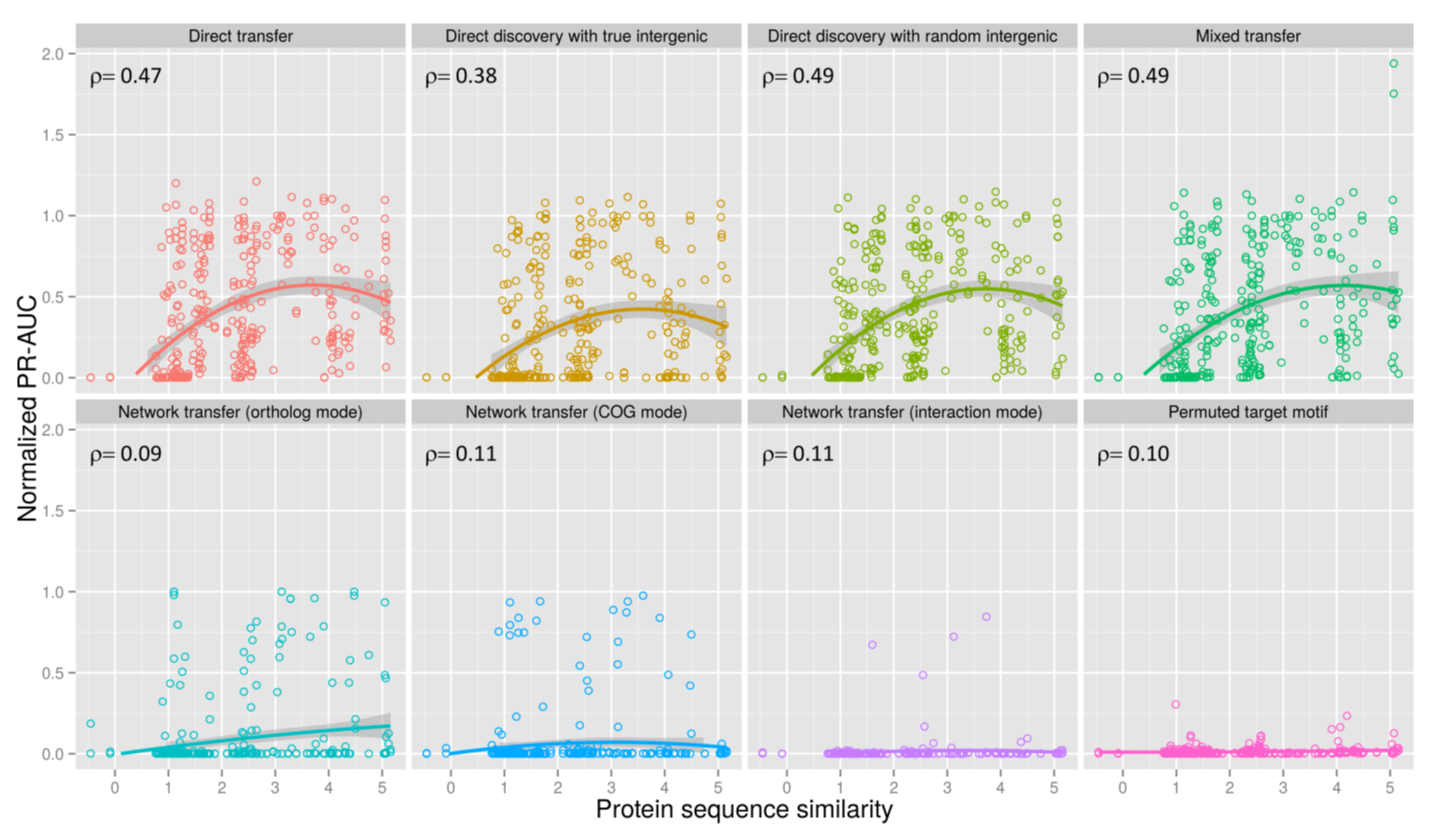
\includegraphics[width=\textwidth]{figures/chapter3/comparison-transfer-methods}
  \caption{Comparison of TRN transfer methods. The plots show the PR-AUC of
    bidirectional transfers between 179 TF-specific species pairs using
    motif-based (direct transfer, direct discovery with true intergenic and
    direct discovery with random intergenic) and transfer-based methods
    (ortholog, COG and interaction modes), as well as a mixed model integrating
    direct transfer and the union of all network-based transfer methods. The
    results obtained with a permutation of the target motif are shown for
    comparison. The x-axis denotes protein similarity as the BLOSUM62 score of
    the ungapped pair-wise alignment between reference and target TF protein
    sequences. PR-AUC values are normalized to the respective AUC of the known
    target TF-binding motif to compensate for the decreased search efficiency
    of low information content motifs. Spearman correlation coefficients
    ($\rho$) of PR-AUC with protein similarity are shown for each case.}
\label{fig:comparison-transfer-methods}
\end{figure}

\begin{figure}
  \centering
  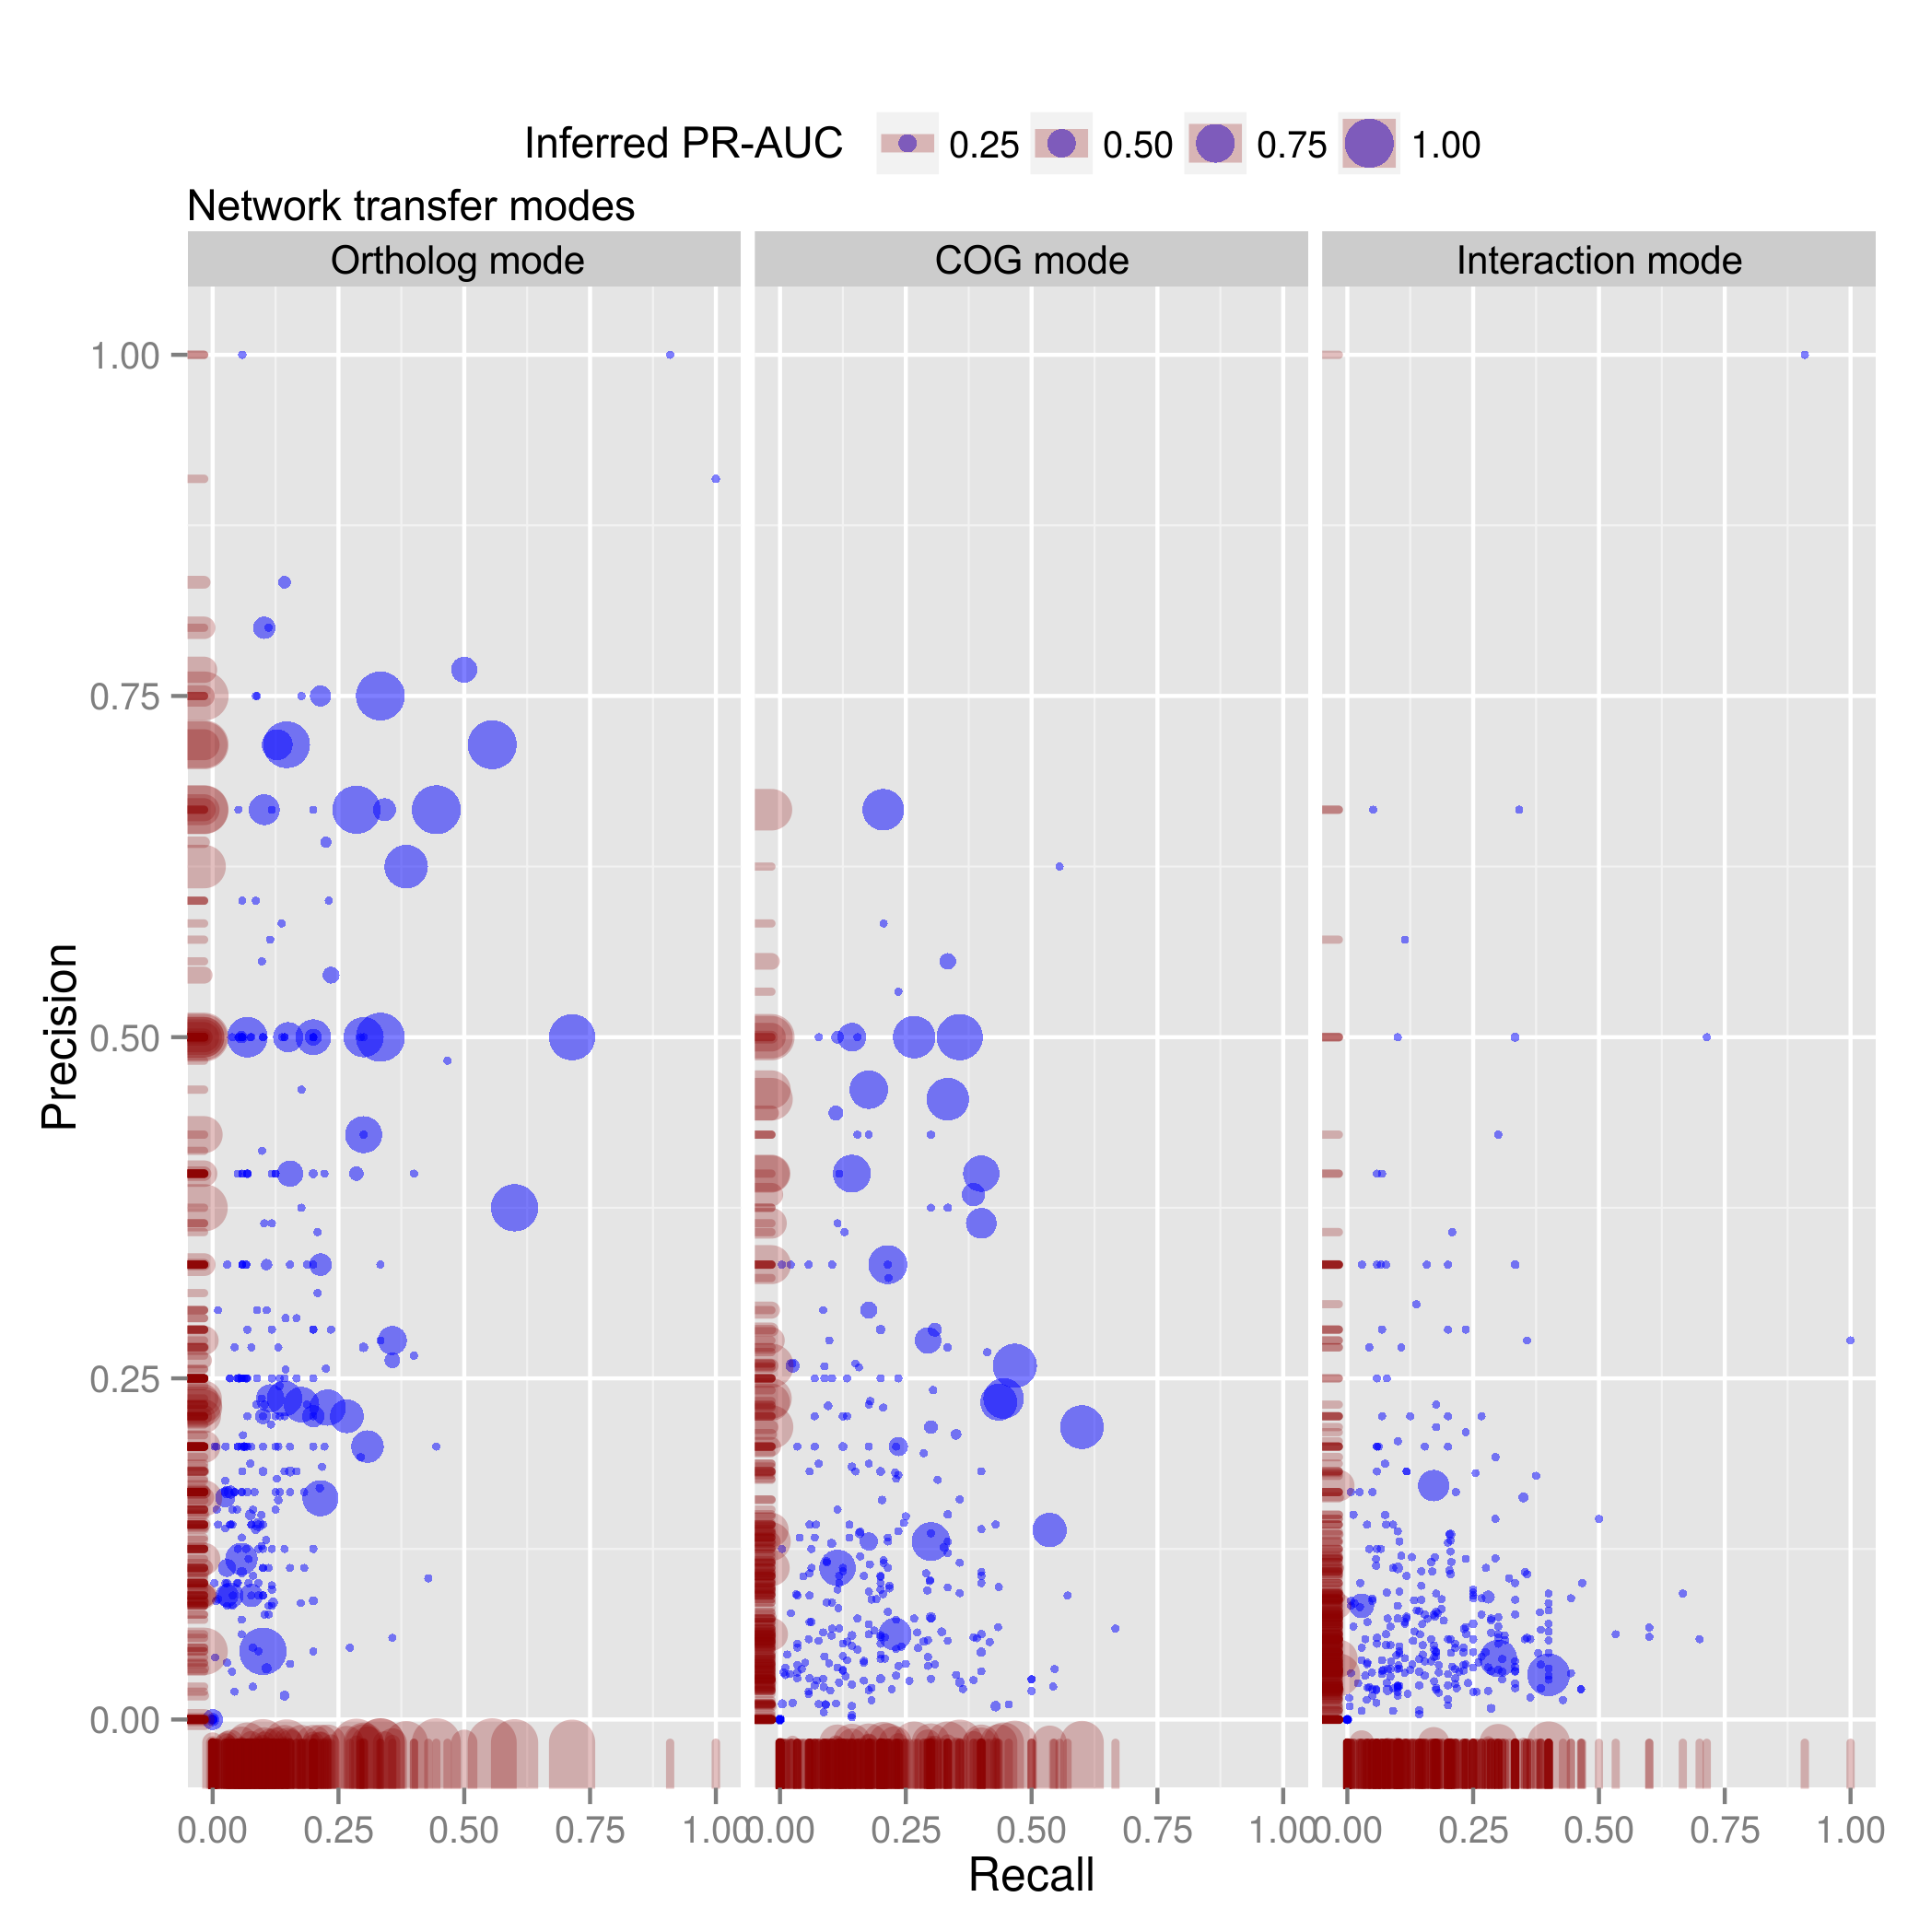
\includegraphics[width=0.9\textwidth]{figures/chapter3/network-transfer-auc}
  \caption{Precision-recall curve for network transfer modes. The plot shows
    the site search PR-AUC of network based transfers as a function of the
    precision and recall of the regulation mapping process. Precision is
    defined as the proportion of mapped genes belonging to the known target
    motif (true positives) with respect to all mapped genes (true and false
    positives). Recall is defined as the proportion of mapped genes belonging
    to the known target motif (true positives) versus the all known target
    motif genes (true positives and false negatives).}
\label{fig:network-transfer-auc}
\end{figure}

In contrast with network-based transfer methods, the different implementations
of motif-based transfer yield very similar results
(Figure~\ref{fig:comparison-transfer-methods}). Using the reference motif to
search promoter regions and define the putative target motif (\textit{direct transfer})
provides results comparable to those obtained with other motif-based transfer
methods and robust with respect to the specific threshold used to define the
motif (Figure~\ref{fig:direct-transfer-alpha}). The use of MEME in \textit{direct
discovery} transfers to rediscover the TF-binding motif, which has been
postulated to refine and better adapt the inferred motif to the target
genome~\cite{habib2012functional}, does not provide significant improvements
over \textit{direct transfer}. In fact, when performing motif discovery in the
promoter region surrounding the identified sites, MEME may identify other
genomic elements (e.g. Pribnow boxes) as the best motifs, decreasing the
accuracy of the method. Performing motif inference on the identified sites
surrounded by random promoter regions prevents this effect but does not yield a
systematic improvement in PR-AUC values over the direct transfer. Finally, the
\textit{mixed mode} approach, which has been associated with enhanced
specificity~\cite{baumbach2010power, baumbach2009reliable}, did not yield a
systematic improvement over direct transfer either.

\begin{figure}
  \centering
  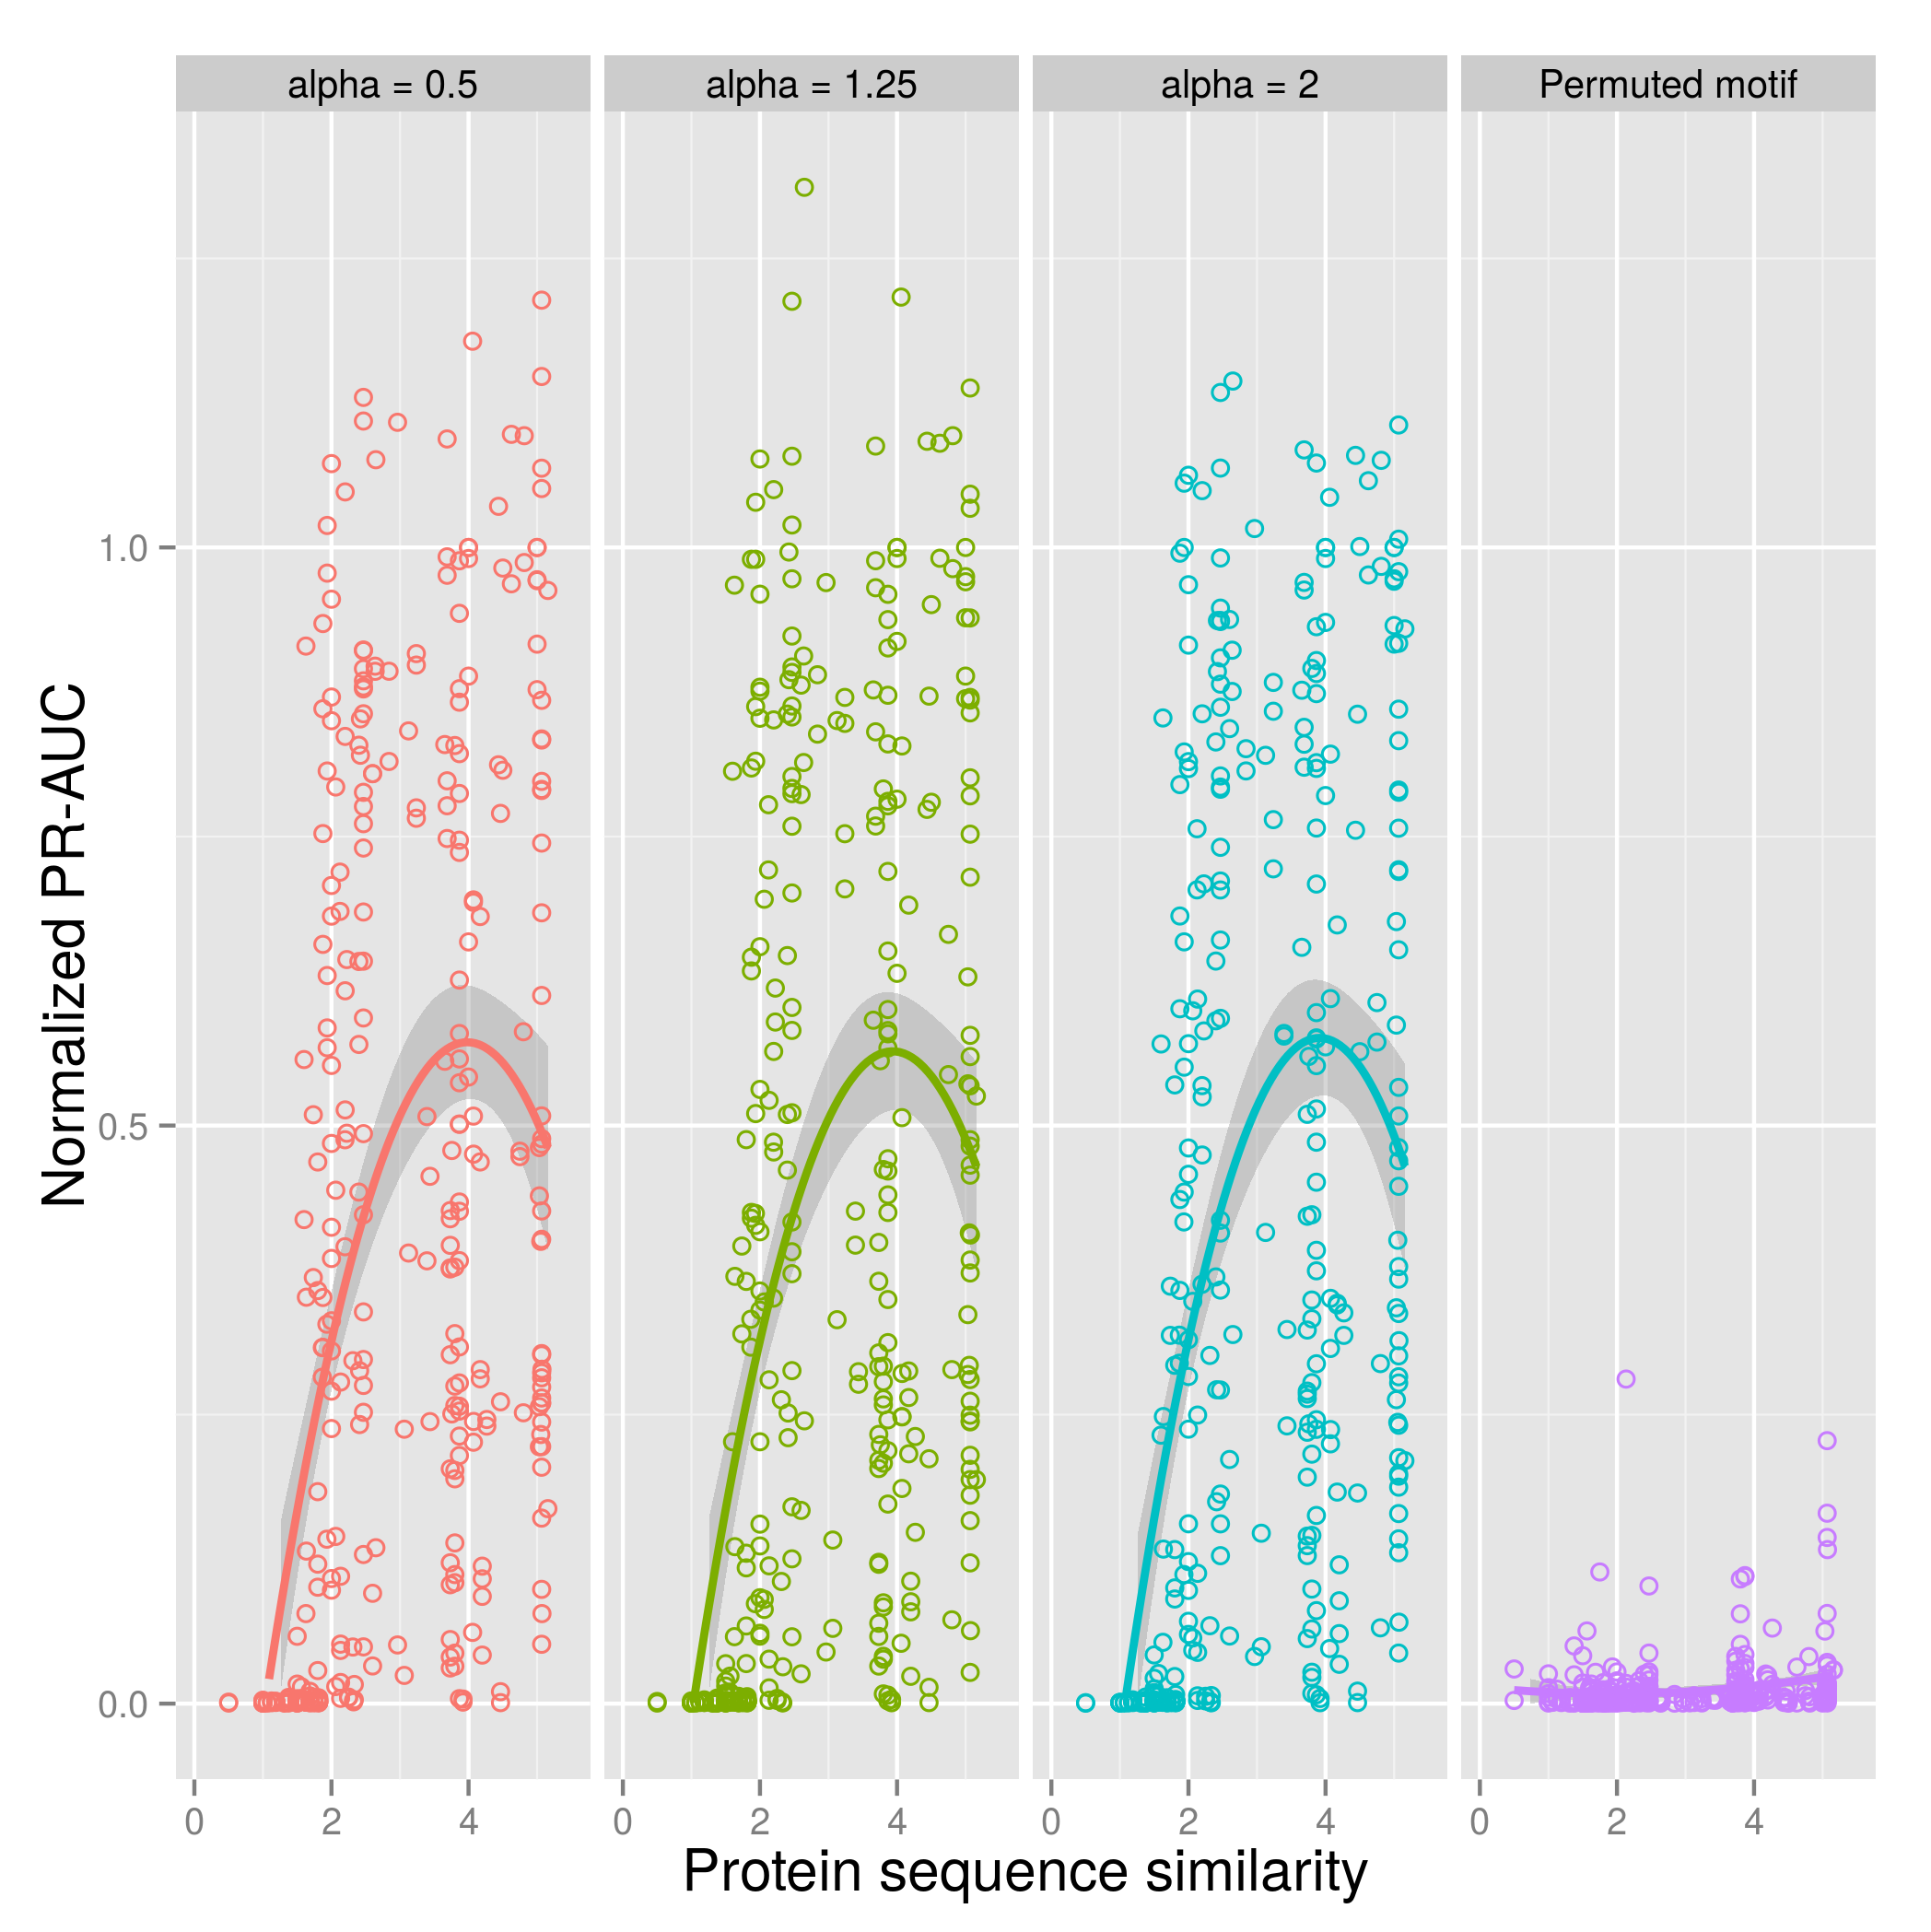
\includegraphics[width=0.9\textwidth]{figures/chapter3/direct-transfer-alpha}
  \caption{Precision-recall curve for direct transfer using different values of
    the scaling factor $\alpha$. The plots show the PR-AUC of bidirectional
    transfers between 179 TF-specific species pairs using the motif-based
    direct transfer method as a function of protein sequence similarity. The
    x-axis denotes protein similarity as the BLOSUM62
    score~\cite{henikoff1992amino} of the ungapped pair-wise alignment between
    reference and target TF protein sequences. PR-AUC values are normalized to
    the respective AUC of the known target TF-binding motif to compensate for
    the decreased search efficiency of low information content motifs. The
    results obtained with a permutation of the target motif are shown for
    comparison.}
\label{fig:direct-transfer-alpha}
\end{figure}

\subsection{Predictive indicators of transfer accuracy}

Our comparative analysis of transfer methods
(Figure~\ref{fig:comparison-transfer-methods}) indicates that even at
relatively close phylogenetic distances, both motif- and network-based transfer
methods may provide inaccurate results. Hence, manual curation of transfer
results, which has been the \textit{de facto} standard for comparative genomics of TRN
in Bacteria~\cite{tan2001comparative, erill2004differences,
  gelfand2000comparative, novichkov2010regpredict}, appears to be a necessary
requisite to ensure the reliability of any subsequent comparative genomics
analyses. Leveraging the TF-binding site catalog compiled here, we attempted to
identify predictive indicators of transfer accuracy for motif- and
network-based transfer methods. Several studies have exploited sequence
similarity in the DNA-binding domain of the TF as a criterion for clustering
putative regulatory regions in motif discovery~\cite{francke2008generic,
  ravcheev2014comparative, dufour2010reconstruction, sahota2010novel}. The
rationale for this approach is that similar DNA-binding domains will target
conserved TF-binding motifs. Hence, it is plausible to assume that DNA-binding
domain sequence similarity could be an efficient predictor of transfer accuracy
for motif-based transfer methods.

To test whether DNA-binding domain sequence similarity is a good predictor of
transfer accuracy, we examined transfer accuracy for two transcription factors
(LexA and Fur) on which we had abundant TF-binding site data and for which the
DNA-binding domain has been experimentally determined
\cite{pohl2003architecture, zhang2010structure}. The results shown in
Figure~\ref{fig:protein-sequence-similarity} reveal that DNA-binding domain
sequence similarity is not a universal predictor of transfer accuracy. For
LexA, DNA-binding domain sequence similarity shows a clear correlation
(Spearman $\rho=0.81$) with motif-based transfer accuracy, but this correlation
is completely absent for Fur ($\rho=0.01$). Our results, therefore, suggest
that for transcription factors (like Fur) targeting a conserved binding motif,
the efficiency of motif-based methods will not significantly decrease with
sequence divergence in the DNA-binding domain. In contrast, and in agreement
with previous findings~\cite{yu2004annotation}, the accuracy of motif-transfer
methods is expected to decrease sharply for LexA and other transcription
factors that have significantly altered their binding specificity through
evolution. In this context, DNA-binding domain sequence similarity provides a
more accurate indicator of transfer efficiency than phylogeny
(Figure~\ref{fig:phylogenetic-distance}).

\begin{figure}
  \centering
  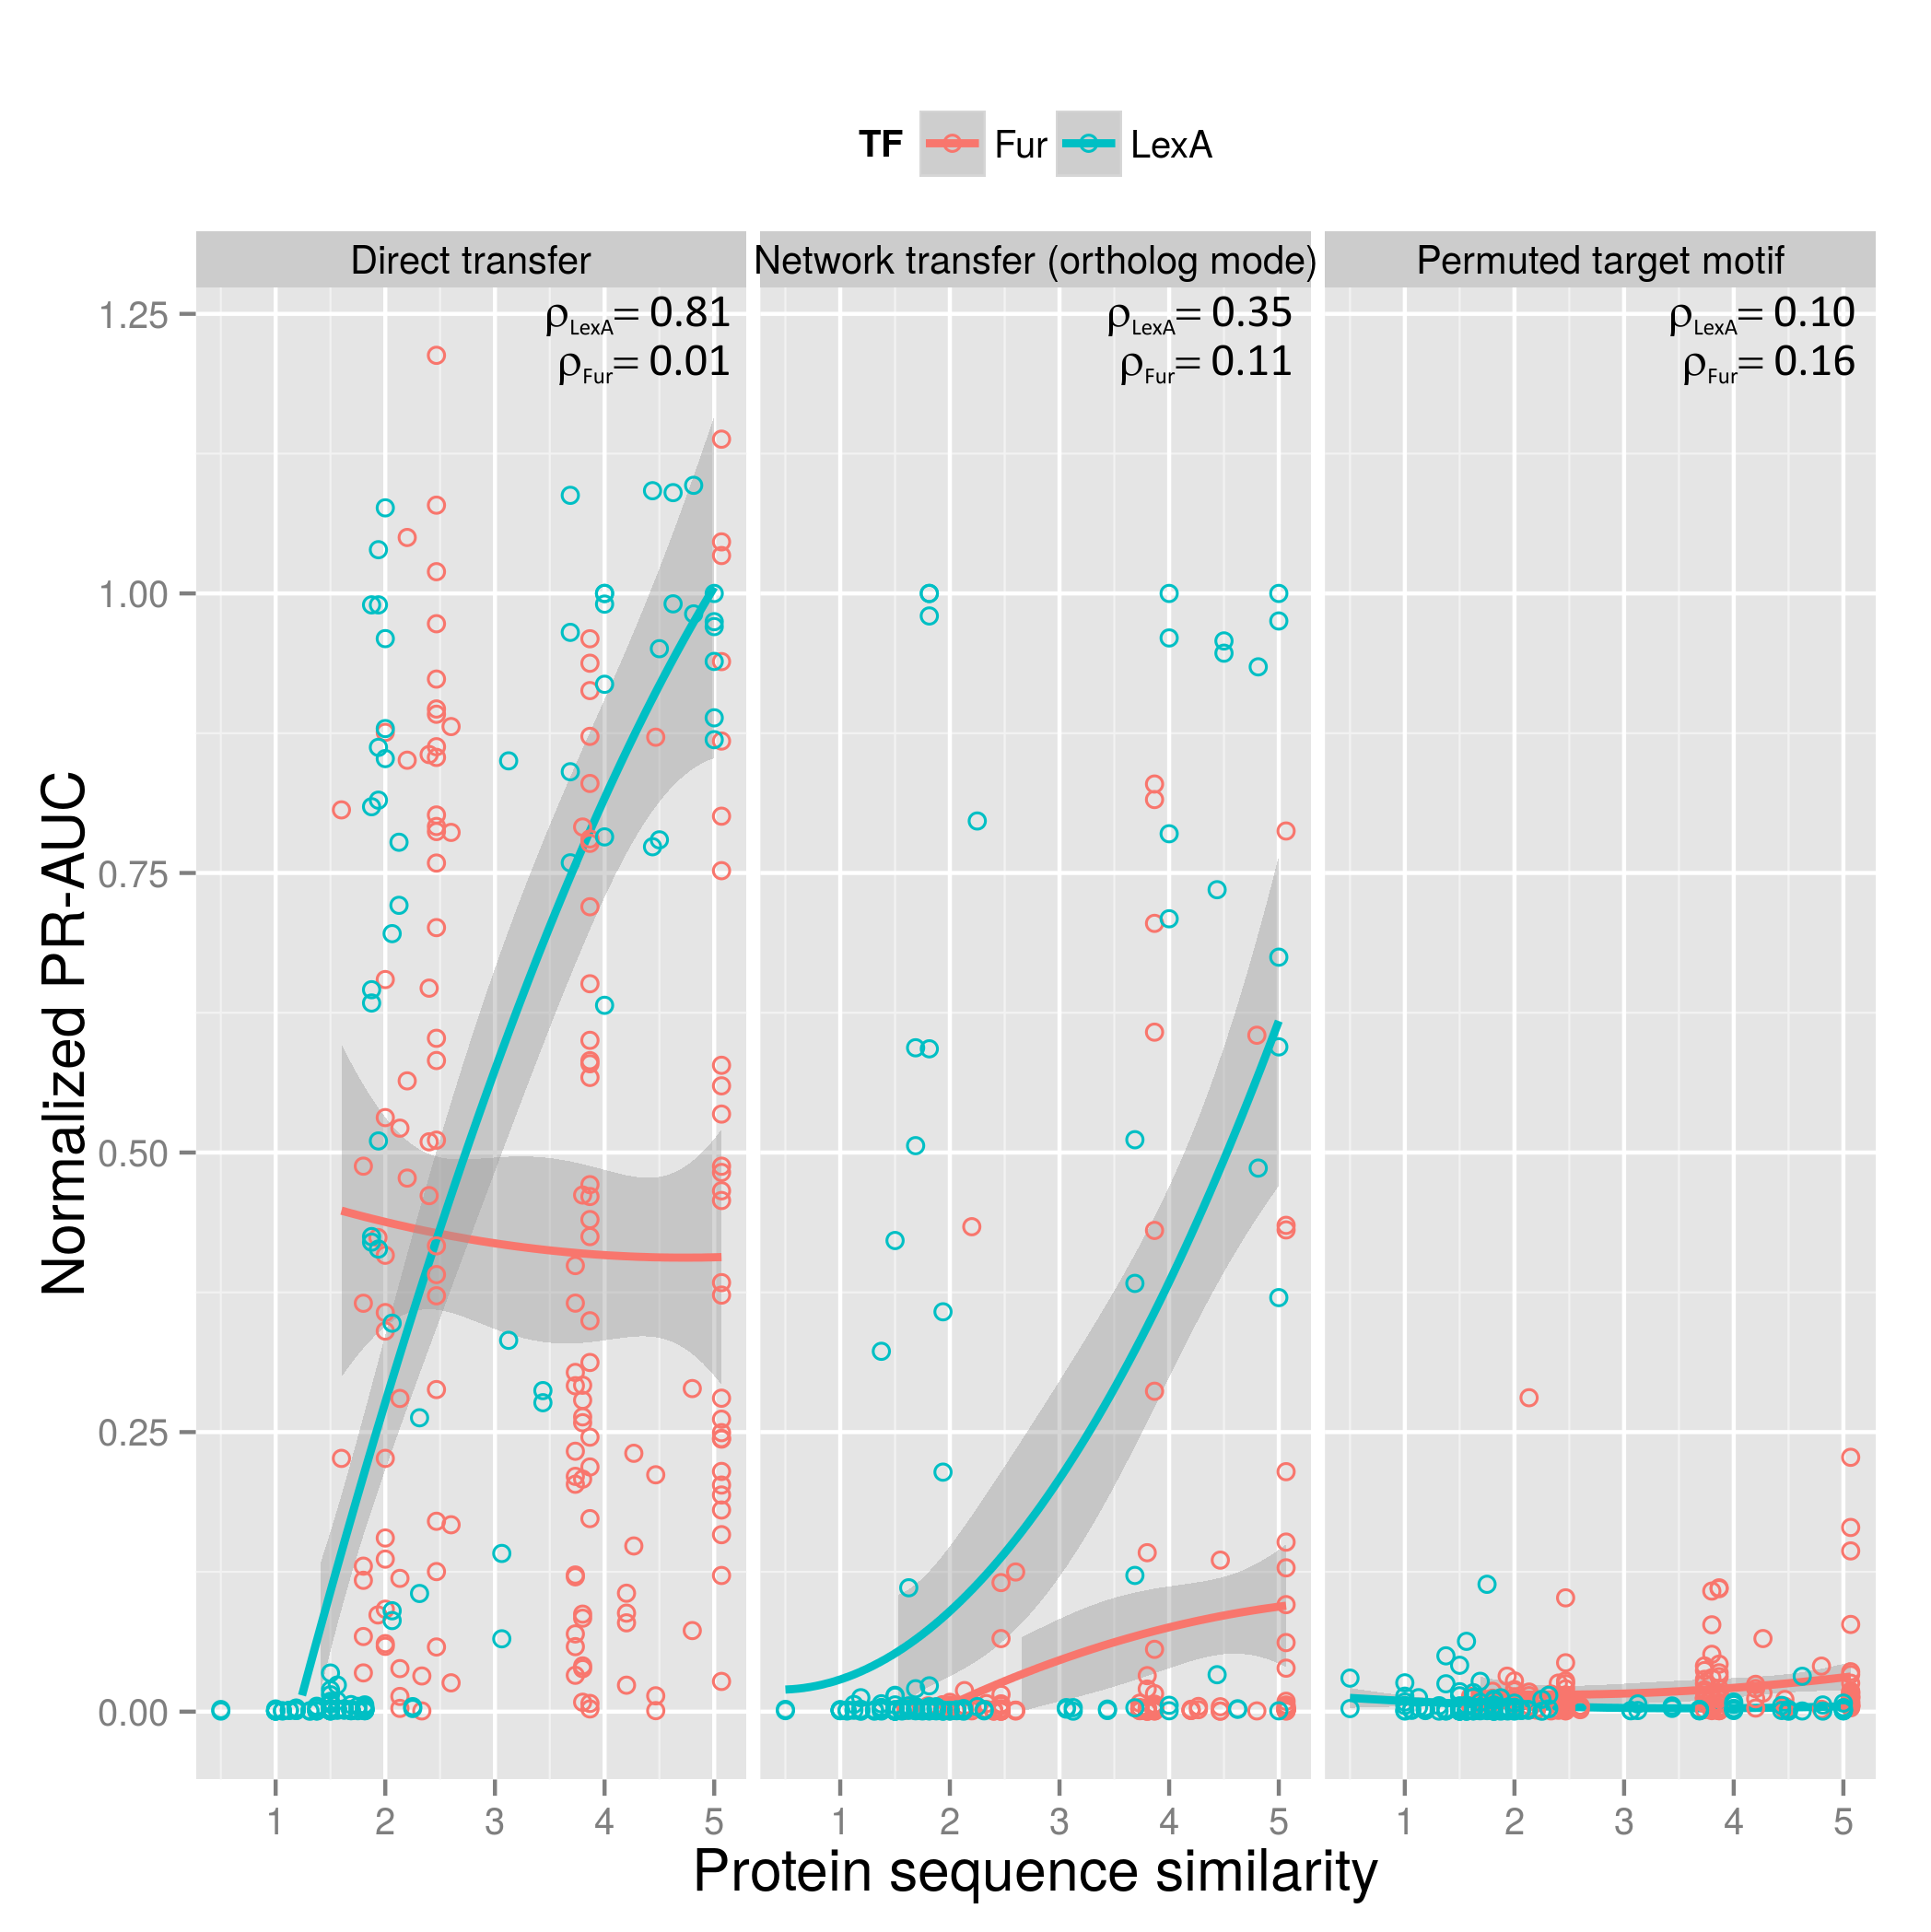
\includegraphics[width=\textwidth]{figures/chapter3/protein-sequence-similarity}
  \caption{Assessment of protein sequence similarity as a predictor of TRN
    transfer method accuracy. The plots show the PR-AUC of bidirectional
    transfers between 143 (66 LexA, 77 Fur) TF-specific species pairs using
    motif-based (direct transfer) and transfer-based methods
    (ortholog mode) as a function of TF protein sequence
    similarity. The results obtained with a permutation of the target motif are
    shown for comparison. The x-axis denotes protein similarity as the BLOSUM62
    score of the ungapped pair-wise alignment between reference and target TF
    protein sequences. PR-AUC values are normalized to the respective AUC of
    the known target TF-binding motif to compensate for the decreased search
    efficiency of low information content motifs. Spearman correlation
    coefficients ($\rho$) of PR-AUC with protein similarity are shown for each
    case.}
\label{fig:protein-sequence-similarity}
\end{figure}

\begin{figure}
  \centering
  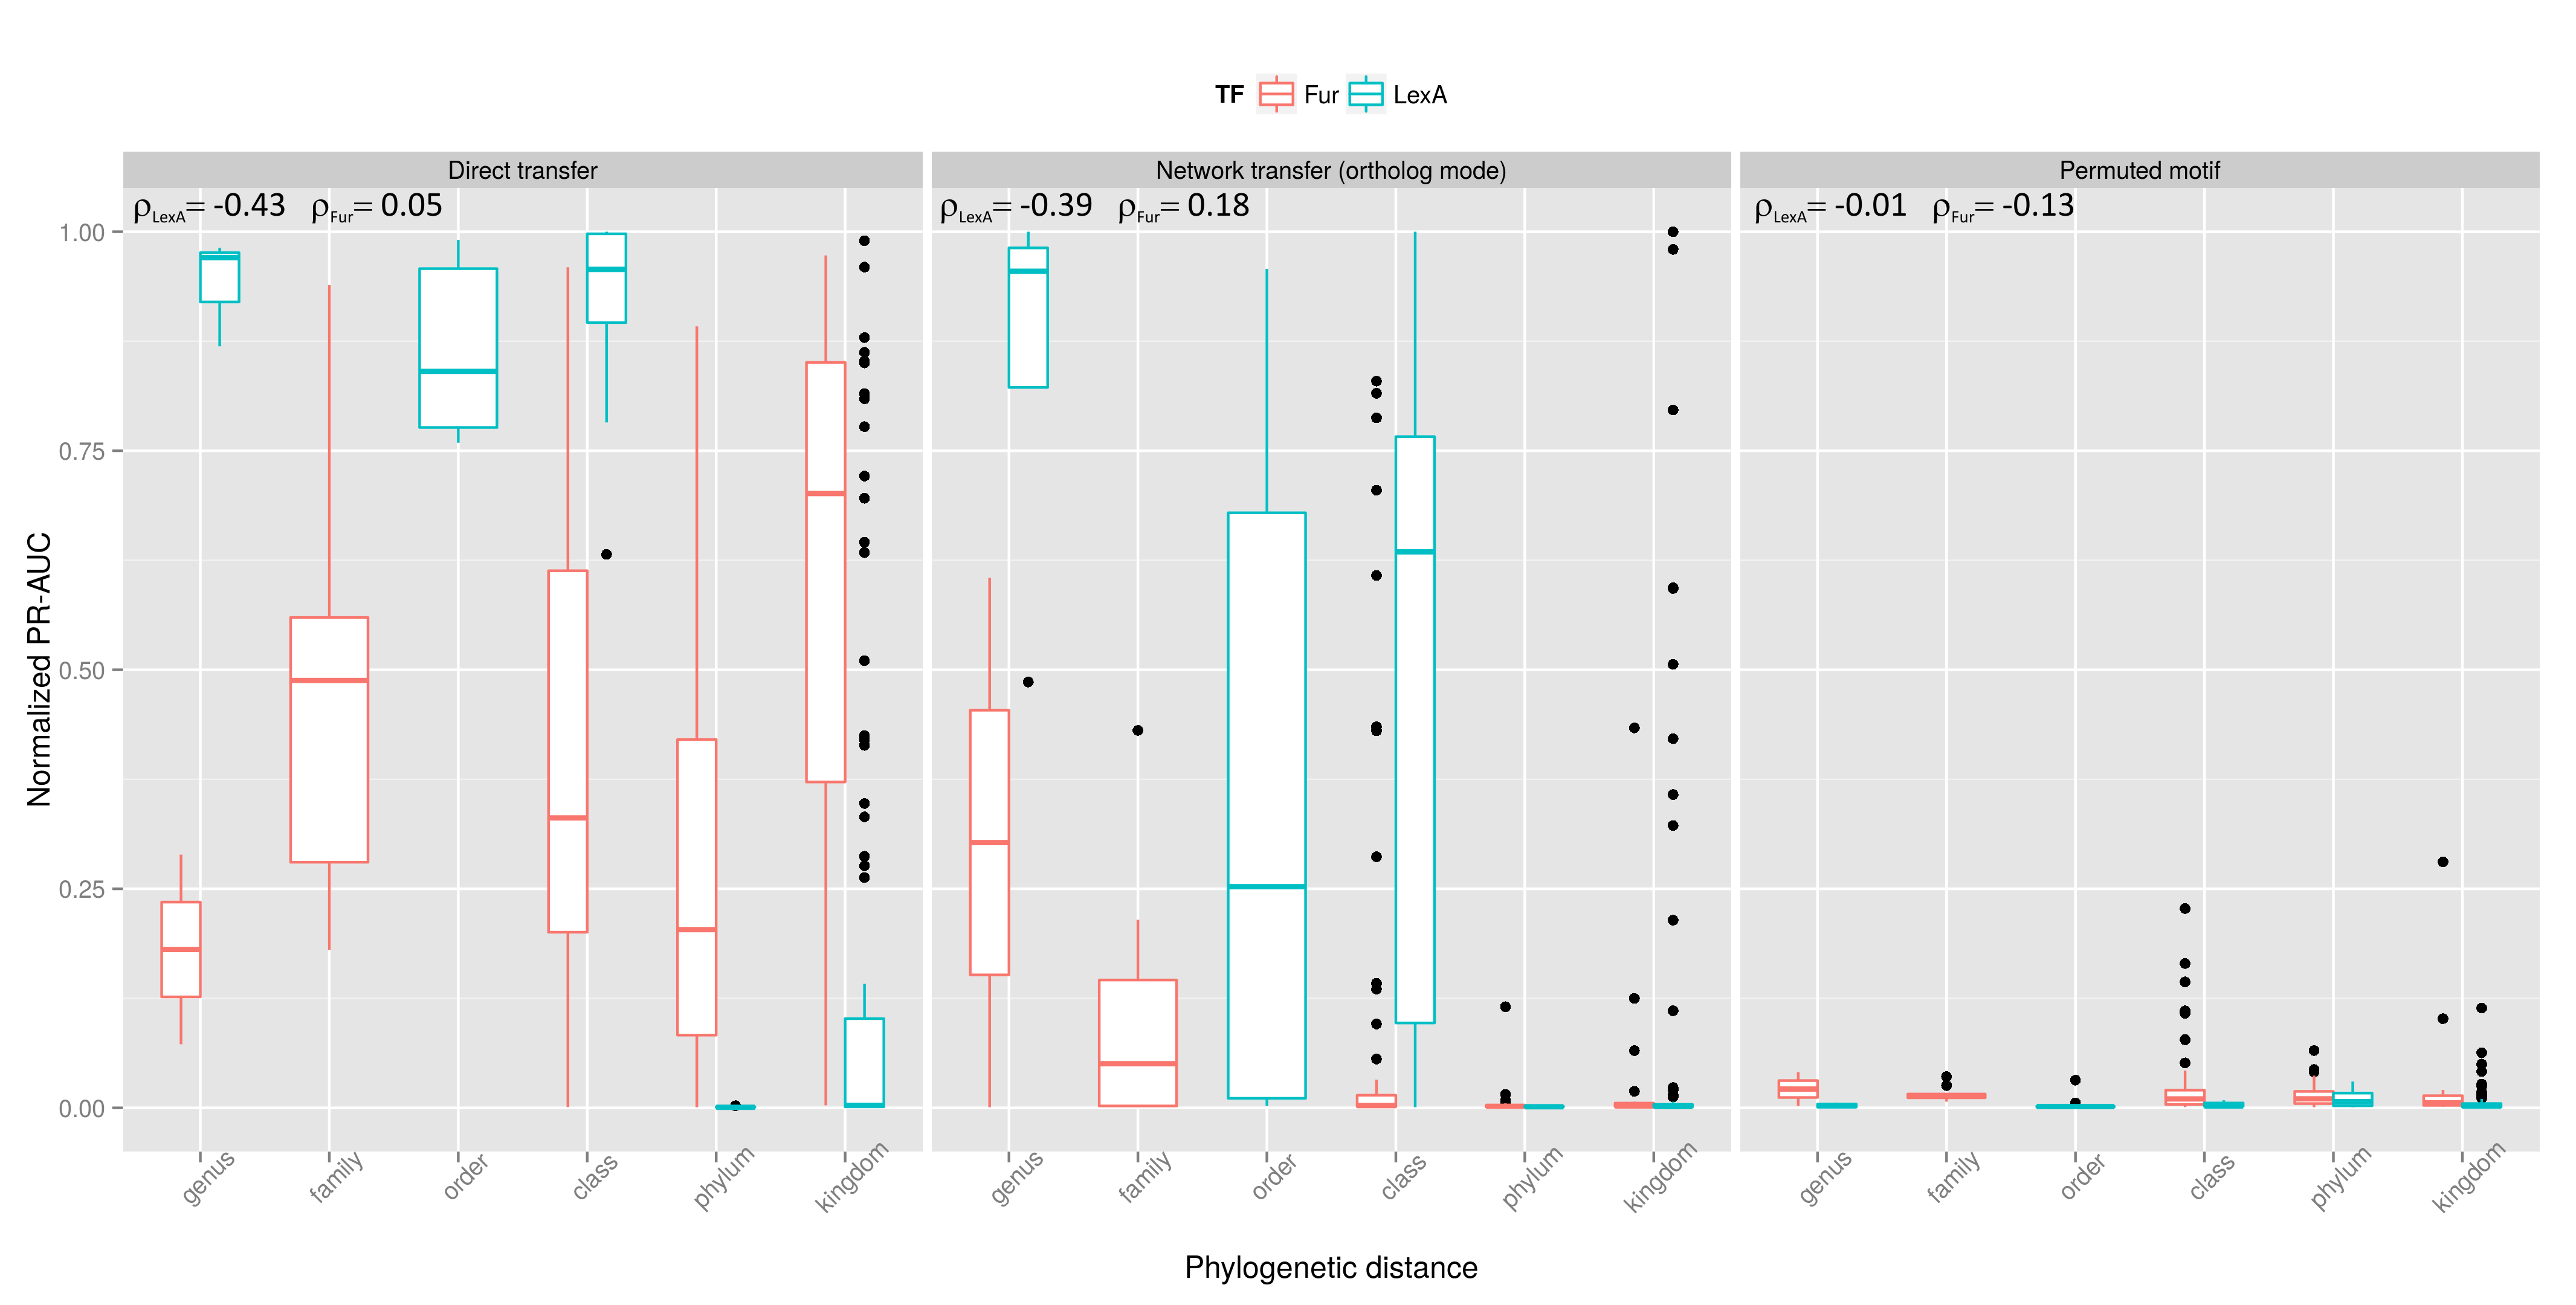
\includegraphics[width=\textwidth]{figures/chapter3/phylogenetic-distance}
  \caption{Box-plot of PR-AUC for motif-based (direct transfer) and
    network-based (ortholog mode) transfer methods summarizing the results of
    bidirectional transfers between 143 (66 LexA and 77 Fur) TF-specific
    species pairs. The x-axis denotes the lowest (more specific) taxonomic
    level shared by the two species. PR-AUC values are normalized to the
    respective AUC of the known target TF-binding motif to compensate for the
    decreased search efficiency of low information content motifs. The results
    obtained with a permutation of the target motif are shown for comparison.}
\label{fig:phylogenetic-distance}
\end{figure}

The results that are shown in Figure~\ref{fig:protein-sequence-similarity} also
indicate that DNA-binding domain sequence similarity correlates weakly with
accuracy for network-based transfer methods. DNA-binding domain sequence
similarity is a proxy for phylogenetic distance
(Figure~\ref{fig:phylogenetic-distance}), and the observed loss of accuracy of
network-based transfer methods is hence congruent with decreased overlap in the
components of regulatory networks for increasing phylogenetic
distances~\cite{venancio2009reconstructing, baumbach2010power,
  price2007orthologous}. It is possible, however, to conceive of other measures
that might function as predictive indices of transfer accuracy for
network-based transfer methods. These methods rely on motif discovery
algorithms, like MEME, to infer the functional motif for the transcription
factor in the target species, providing some theoretical bounds on expected
properties of the inferred motifs. For instance, the information content (IC)
of a TF-binding motif is known to correlate with the number of operons
regulated by the TF~\cite{schneider1986information}. Hence, if the size of the
regulatory network is assumed to remain relatively constant, we expect the IC
of the inferred TF-binding motif to be similar to that observed in the
reference species. In a similar vein, the distribution of information in a
TF-binding motif is related to the structure of the TF and its mode of binding
(e.g.\ homodimers typically target palindromic
motifs)~\cite{ravcheev2014comparative, gelfand1999recognition,
  schneider1996reading}. It follows that measures of information distribution
in inferred TF-binding motifs, such as the Gini
coefficient~\cite{dorfman1979formula}, should not differ much between the
reference and inferred motifs under the assumption of conserved protein
structure. We analyzed the predictive power of these indices on PR-AUC using
the complete TF-binding site catalog (Figure~\ref{fig:ic-and-gini}). While
neither index can reliably identify successful transfers, both indices reveal
clear cutoff values beyond which accurate transfers should not be expected. For
both IC and Gini coefficient, a relative index of 0.5 with respect to the known
reference motif is a strong indicator of unsuccessful transfer (96\% and 94\%
unsuccessful transfers for IC and Gini relative values below 0.5, compared to
83\% for both IC and Gini values above 0.5), and the evidence suggests that
this may also be true for IC and Gini values above 2.

\begin{figure}
  \centering
  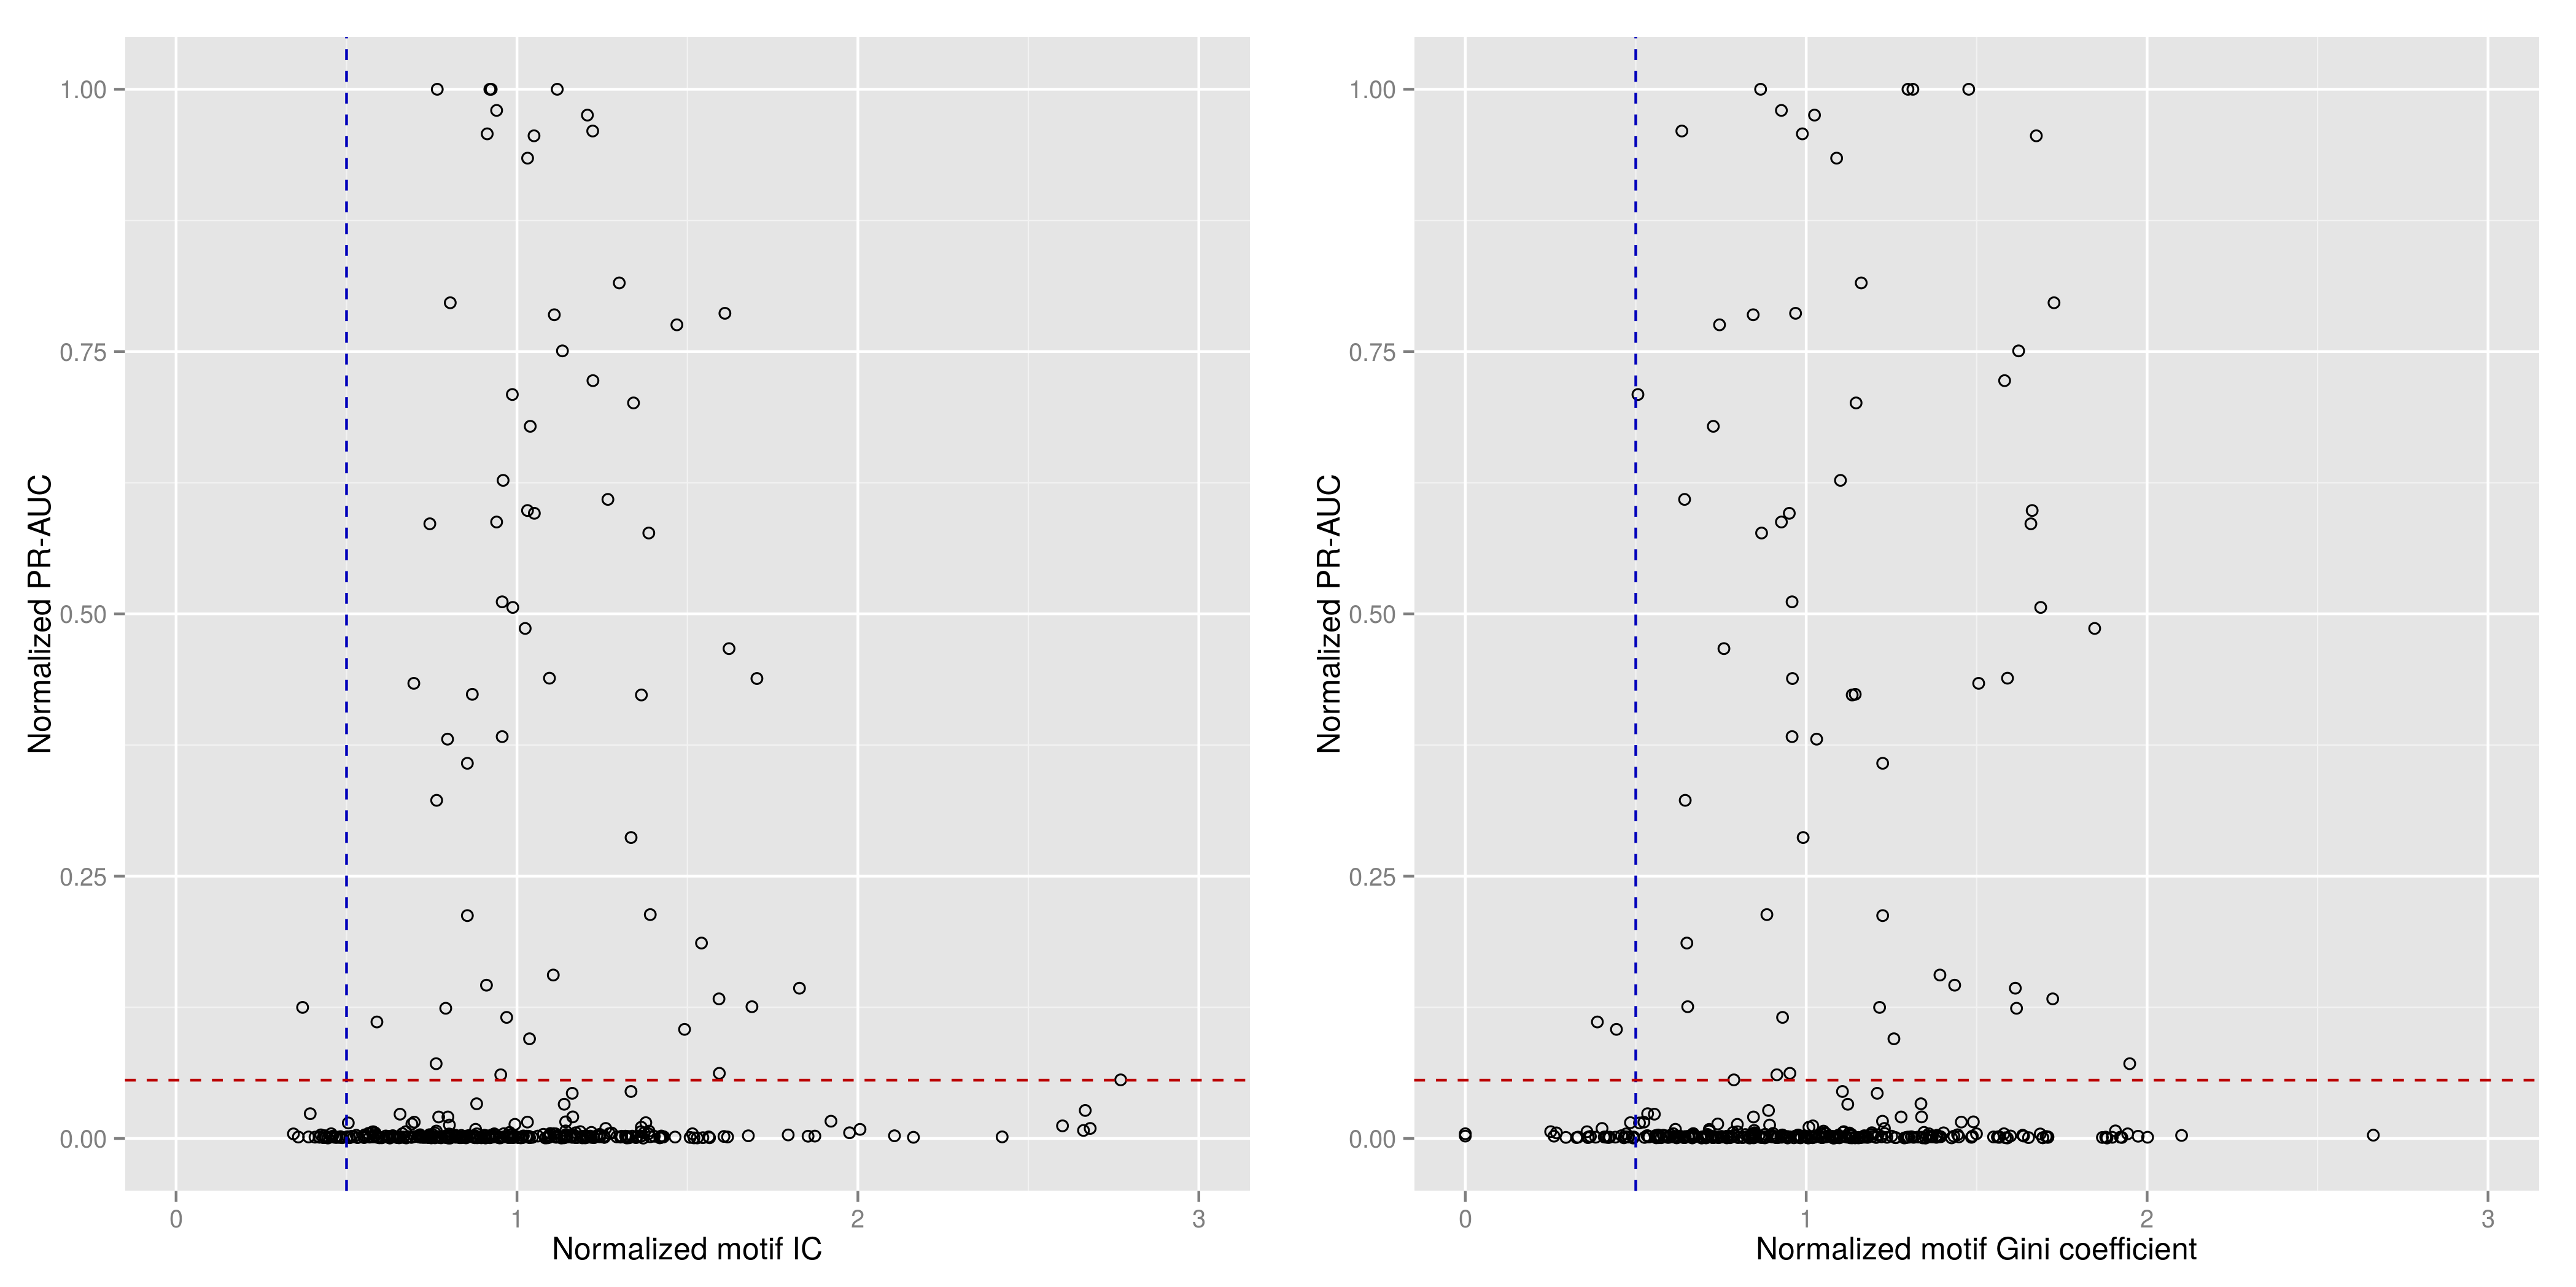
\includegraphics[width=\textwidth]{figures/chapter3/ic-and-gini}
  \caption{Assessment of IC (left) and Gini coefficient (right) as predictive
    indices of accuracy for network-based transfer methods. The plots show the
    distribution of PR-AUC from bidirectional transfers between 179 TF-specific
    species pairs using network transfer (ortholog mode), with respect
    to each index. PR-AUC values are normalized to the respective AUC of the
    known target TF-binding motif to compensate for the decreased search
    efficiency of low information content motifs. IC and Gini coefficient
    values are normalized to those observed on the known reference motif. The
    dotted vertical line designates 0.5 normalized motif IC/Gini. The dotted
    horizontal line identifies the PR-AUC value (0.056) two standard deviations
    above the mean obtained from simulated transfers with permuted motifs.
  }
\label{fig:ic-and-gini}
\end{figure}

\section{Conclusions}

Transferring known information about transcriptional regulatory networks from
reference to target species is a critical step in comparative genomics
analyses. In this work, we compiled a catalog of known TF-binding sites in
Bacteria and performed a methodic evaluation of assessment metrics in order to
perform the first systematic analysis of different transfer methods. Our
results identify the precision-recall area-under-the-curve as the most reliable
metric for transfer efficiency. We also show that motif-based transfer methods
dramatically outperform network-based approaches, but their effectiveness may
decrease sharply with increasing phylogenetic distance. We evaluate some
predictive indicators of transfer accuracy and show that they are not
consistent or precise enough to enable full automation of TRN transfer. Our
results hence support the long-standing practice of manual curation in
comparative genomics analyses and reveal that the introduction of more
elaborate methods does not clearly benefit motif- or network-based transfer
approaches.

\section{Methods}

\subsection{TF-binding site and genome data}

Experimentally-validated TF-binding sites were compiled from CollecTF
\cite{kilic2013collectf}, a Bacteria domain-wide TF-binding site database, and
four model-organism databases: RegulonDB, CoryneRegNet, DBTBS and MtbRegList
\cite{jacques2005mtbreglist, sierro2008dbtbs, pauling2012coryneregnet,
  salgado2013regulondb}. Data from these databases was downloaded and merged
after removal of duplicates and data without supporting experimental
evidence. To evaluate transfer methods across pairs of species, only regulons
with at least 10 experimentally-validated TF-binding sites for a given TF in
both species were used. Complete genome sequences and annotations for species
with available TF-binding site data were downloaded from the NCBI RefSeq
database~\cite{pruitt2007ncbi}. Operon predictions for all genomes and COG
annotations for protein-coding genes were obtained from the DOOR database
\cite{tatusov2000cog, mao2009door}.

\subsection{TF-binding site search and motif discovery}

For TF-binding site search, only the regions spanning from -300 bp to +50 bp
relative to the corresponding gene translation start site were considered. Site
search was implemented using custom scripts based on standard Biopython library
functions~\cite{cock2009biopython}. The searched regions were scanned with a
sliding window, evaluating each position with a position-specific scoring
matrix (PSSM) based on a uniform background mononucleotide model
\cite{stormo2000dna}. Motif discovery on selected sequences was performed with
MEME, using command line settings \texttt{-zoops -revcomp -dna}, and maximum
and minimum motif widths, respectively, of 150\% and 50\% of the reference
motif width~\cite{bailey2015meme}.

\subsection{Transfer methods}

Two main motif-based transfer methods were implemented. In the direct transfer,
a position-specific scoring matrix (PSSM) is built from the reference
collection of binding sites and used to scan the promoter regions of the genome
of interest to identify putative sites~\cite{stormo2000dna}. Under the
assumption that regulon size is conserved to a first approximation, the target
motif is defined as composed of the highest scoring $N_T$ sites.
$N_T = \alpha \cdot N_R \cdot G_T/G_R$, where $N_R$ is the number of sites in
the reference species, $G_T$ and $G_R$ are genome lengths for target and
reference species, respectively, and is used as a scaling factor to modulate
specificity ($\alpha=1.25$). Direct discovery uses a relaxed scaling factor
($\alpha=2.50$) to generate a larger collection of putative sites. These sites
and their adjoining intergenic regions are used to rediscover the TF-binding
motif with MEME in direct discovery with true intergenic. For direct discovery
with random intergenic, the genomic intergenic regions are substituted by 100
bp stretches randomly generated following the intergenic region nucleotide
frequencies.

The network-based transfer was implemented using three different criteria to
map regulated genes in the reference genome to target genomes. In ortholog
mode, orthologs of all genes belonging to regulated operons were detected as
best reciprocal BLAST hits between species pairs using a minimum e-value
threshold of $10^{-10}$~\cite{moreno2008choosing}. In COG mode, all genes in the
target genome mapping to the same COG as genes in regulated operons of the
reference genome were considered functional orthologs. In interaction mode,
direct interacting partners for regulated genes in the reference genome were
identified using the STRING database~\cite{franceschini2013string}. The
orthologs of these genes on target genomes were detected through reciprocal
BLAST and used to define putative regulatory networks. In all three cases, the
promoters of all target operons containing mapped genes were then used for
motif discovery with MEME\@.


Mixed transfer uses a relaxed ($\alpha=2.50$) TF-binding site search with the
reference TF-binding motif to define a set of putative sites in the target
genome. This collection of putative sites is filtered by retaining only those
sites next to operons containing genes that have been mapped to the target
genome by any of the network-based transfer methods.

\subsection{Assessment metrics}

Two main types of assessment metrics were used to gauge the efficacy of TF
motif-based transfer methods: motif comparison and performance metrics. Motif
comparison methods involve the direct comparison of the TF-binding motifs
inferred by the transfer method and the motif generated from the known
collection of regulated genes in the target genome. To compare motifs of
different lengths, the two collections of binding sites are shifted with
respect to each other to obtain the gapless alignment that maximizes the
information content (IC) of the joint collection
\cite{schneider1986information}. The aligned region of each collection is then
used to compute its position-specific frequency matrix (PSFM). The similarity
between the two PSFM is evaluated using either the Euclidean distance or the
Kullback–Leibler (KL) divergence of the inferred motif from the known target
motif~\cite{gupta2007quantifying}. Performance metrics evaluate the ability of
the inferred motif to retrieve the known target sites when searching an equal
number of promoter regions from the target genome containing, and not
containing, known sites. To assess true positives, the maximum IC alignment
between target and inferred collections is used to compute the offset between
predicted and known sites. The accuracy of the search using the inferred
TF-binding motif is then evaluated as the area-under-the-curve (AUC) of the
receiver-operator-characteristic (ROC) or precision-recall (PR) curve, computed
with the scikit-learn Python library functions~\cite{lewis1991evaluating,
  zweig1993receiver, scikit-learn}.

Control experiments for TRN transfer were generated in two different
ways. Noisy transfers were simulated by defining the inferred motif as a
mixture pseudoreplicate of the known target collection and sequences from the
promoter region of the target genome. Given a mixture weight $\omega$, the
pseudoreplicate is obtained by sampling, with replacement, $(1-\omega) \cdot N$
sites from the known target collection and $\omega \cdot N$ sequences of length
$L$ from the promoter region of the target genome (where $N$ and $L$ are,
respectively, the number and width of sites in the known target collection)
(Figure~\ref{fig:transfer-methods}). Noisy transfers were generated for 0.1,
0.25, 0.5 and 0.75 values of $\omega$, simulating increasingly inefficient
transfers. Permuted transfers were obtained by randomly sampling, without
replacement, the columns of the known target motif. A transfer was considered
successful if its PR-AUC was larger than two standard deviations above the mean
PR-AUC value observed for permuted transfers.
